\subsection{Results and discussion}

%%%%%%%%%%%%%%%%%%%%%%%%%%%%%%%%%%%%%%%%%%%%%%%%%%%%%%%%%%%%%%%%
%%  PocketVec performance on the ProSPECCTs benchmark sets  %%%%
%%%%%%%%%%%%%%%%%%%%%%%%%%%%%%%%%%%%%%%%%%%%%%%%%%%%%%%%%%%%%%%%

\phantomsection
\subsubsection{PocketVec performance on the ProSPECCTs benchmark sets}
\label{PocketVec_ResultsAndDiscussion_PocketVec_performance_on_the_ProSPECCTs_benchmark}

The performance of PocketVec descriptors across ProSPECCTs datasets is assessed in terms of the AUROC and is shown in Fig \ref{PocketVec_Fig1}d. We observe that PocketVec descriptors are robust to varying definitions of the same pocket, as determined by different crystallized ligands (P1, AUROC 0.97). When restricting such definitions to chemically similar ligands, the performance is maximal (P1.2, AUROC 1.00). Similarly, our descriptors are robust against protein conformational changes, i.e. protein flexibility (P2, AUROC 0.96), and they are also able to distinguish identical pockets from those altered by 5 artificial mutations leading to changes in physicochemical and shape properties of pocket-lining residues. In these cases, we obtained more modest performances (P3--physicochemical changes and P4--both physicochemical and shape changes, AUROCs of 0.67 and 0.72, respectively). Reassuringly though, we observed a significant correlation between the number of artificial mutations (1 to 5) and the corresponding AUROC values (Pearson CC > 0.98, p-value < 0.005 in both P3 and P4, Fig \ref{PocketVec_FigS9}), which confirmed that an increasing number of mutations in the binding site came along with an improved ability to detect such differences using PocketVec descriptors. 

We also benchmarked our descriptors in more biologically relevant scenarios where, for instance, pockets binding similar small molecules are found in structurally different proteins. ProSPECCTs includes two datasets to address such cases: P5 includes pocket structures classified into 9 distinct ligand classes (e.g. HEM, ATP, NAD, etc.), and P7 includes a realistic set of binding site pairs reported to be similar in published literature, some of them identified in otherwise unrelated proteins. In these sets, PocketVec descriptors show performances with AUROCs of 0.64 and 0.87, respectively, demonstrating their ability to identify similar pockets in globally dissimilar proteins. It is important to note that two binding sites having identical (or chemically similar) crystallized ligands are not necessarily similar from a PocketVec perspective. Following the logic behind the similarity ensemble approach (SEA\cite{keiser_relating_2007}), in which targets are quantitatively compared based on the chemical similarity of the ensemble of their ligands, a pair of targets sharing a single active compound may not be significantly similar.

Finally, with the goal of defining a PocketVec distance threshold to classify any pocket pair of interest as either similar or dissimilar, we analyzed the behavior of the Matthew's Correlation Coefficient (MCC) at multiple cut-off values across the different ProSPECCTs datasets (Fig \ref{PocketVec_FigS10}). As expected, each definition of pocket similarity in the ProSPECCTs datasets suggested the choice of a different cut-off distance. For instance, the optimal cut-off in the mutation-related benchmarks (P3 and P4) was around 0.13, while in the most realistic set of binding site pairs reported to be similar in published literature was even lower, around 0.08. However, for general purposes and to minimize false negatives, we selected the distance threshold based on the P1 dataset, where similar pairs were predefined as identical pockets binding chemically distinct ligands whereas dissimilar pairs were unrelated pockets binding different ligands. In this way, we defined 0.17 as our PocketVec threshold distance, which was the value maximizing the MCC in ProSPECCTs P1. However, this threshold should not be regarded as an absolute standard, but rather as a general guideline for classifying a pocket pair of interest as either similar or dissimilar.

For the sake of completeness, we generated results for all combinations of docking methods (rigid--rDock, and flexible--SMINA) and reduced sets of chemical compounds (128 LLM and 128 fragments). The use of rDock and LLM (128) was still the best strategy according to the ProSPECCTs datasets (Fig \ref{PocketVec_FigS11}). Besides, we observed that the selection of compounds leading to the most variable results throughout the different pockets (i.e. high entropy) was, indeed, of great help to distinguish similar from dissimilar pockets in ProSPECCTs P1. This effect was even more pronounced in the fragments, where their lower complexity and molecular weight led to higher promiscuity and redundancy (Fig \ref{PocketVec_FigS12}).

Detailed plots for all ProSPECCTs datasets including ROC Curves, PR Curves and distributions of PocketVec distances, docking scores and pocket volumes are included in our \hl{GitLab repository} (see \hyperref[PocketVec_Code]{Code and data availability}). 



%%%%%%%%%%%%%%%%%%%%%%%%%%%%%%%%%%%%%%%%%%%%%%%%%%%%%%%%%%%%%%%%
%%%%%%%%%%  Comparison with existing strategies  %%%%%%%%%%%%%%%
%%%%%%%%%%%%%%%%%%%%%%%%%%%%%%%%%%%%%%%%%%%%%%%%%%%%%%%%%%%%%%%%

\phantomsection
\subsubsection{Comparison with existing strategies}
\label{PocketVec_ResultsAndDiscussion_Comparison_with_existing_strategies}

Next, we compared the performance of PocketVec descriptors with state-of-the-art methodologies, as reported in several studies\cite{simonovsky_deeplytough_2020, scott_classification_2022, ehrt_benchmark_2018}, where the authors benchmarked many pocket comparison tools against the ProSPECCTs datasets, including six strategies based on pocket descriptors (Fig \ref{PocketVec_Fig1}d and Fig \ref{PocketVec_FigS11}). We used the AUROC as the standard performance measure to be able to compare our results with other available methodologies. However, for PocketVec descriptors, we also provide specific values of precision, accuracy, sensitivity, specificity, Matthew´s correlation coefficient and F1 score in each ProSPECCTs dataset (Fig \ref{PocketVec_FigS13}). Overall, PocketVec is the second-best ranked strategy in terms of the weighted average among datasets (0.89) and, indeed, it surpasses the median and the average performance in all ProSPECCTs datasets, apart from P3 (Table \ref{PocketVec_TableS1}). The top-scoring method is SiteAlign\cite{schalon_simple_2008}, which is alignment-dependent and based on the projection of residue descriptors into a triangle-discretized sphere that quantifies binding site similarity by minimizing distances between systematically generated cavity fingerprints obtained by moving one binding site with respect to the other. Thus, being specifically developed to compare pockets, it does not provide a unique descriptor for each binding site, which hampers the exploration of the pocket space in the same way molecular fingerprints do for the chemical space of small molecules. \hl{START} Other strategies are indeed alignment-free and provide unique representations for binding sites but, in addition to showing worse performances than PocketVec descriptors among ProSPECCTs datasets, also present several intrinsic limitations. For instance, KRIPO\cite{wood_pharmacophore_2012} and TIFP\cite{desaphy_encoding_2013} characterize protein-ligand binding interactions between receptors and bound ligands, which enables the identification of shared interaction patterns between pockets but limits their applicability domain to \textit{holo} structures. Additionally, FuzCav\cite{weill_alignment-free_2010} fingerprints count for specific pharmacophoric triplets of pocket-lining Cα, which enables the use of \textit{apo} structures but imply a simplistic representation of pockets. On a different note, Deeplytough\cite{simonovsky_deeplytough_2020} and BindSiteS-CNN\cite{scott_classification_2022} generate pocket descriptors by means of deep learning strategies, which makes them strongly dependent on training data and provide pocket embeddings that are difficult to interpret. \hl{END} Thus, overall, PocketVec represents a fast strategy to generate accurate pocket descriptors that overcome the aforementioned limitations, and it shows a higher performance at assessing pocket similarities than most current strategies (Fig \ref{PocketVec_FigS14}).




%%%%%%%%%%%%%%%%%%%%%%%%%%%%%%%%%%%%%%%%%%%%%%%%%%%%%%%%%%%%%%%%
%%% Comprehensive characterization of druggable pockets in the human proteome
%%%%%%%%%%%%%%%%%%%%%%%%%%%%%%%%%%%%%%%%%%%%%%%%%%%%%%%%%%%%%%%%

\phantomsection
\subsubsection{Comprehensive characterization of druggable pockets in the human proteome}
\label{PocketVec_ResultsAndDiscussion_Comprehensive_characterization}

PocketVec descriptors constitute an optimal framework to comprehensively characterize large and diverse sets of small molecule binding sites (\textit{apo}/\textit{holo} structures), enabling the navigation across the pocket space of complete proteomes. In view of this, we designed a computational pipeline to generate PocketVec descriptors for all pockets included within human protein domains (Fig \ref{PocketVec_Fig2}a). Please, see \hyperref[PocketVec_Methods]{Methods} for a detailed description of the strategy.

%%%%%%%%%%%%%%%%
%%% FIGURE 2 %%%
%%%%%%%%%%%%%%%%


\begin{figure}[H]
  \centering
  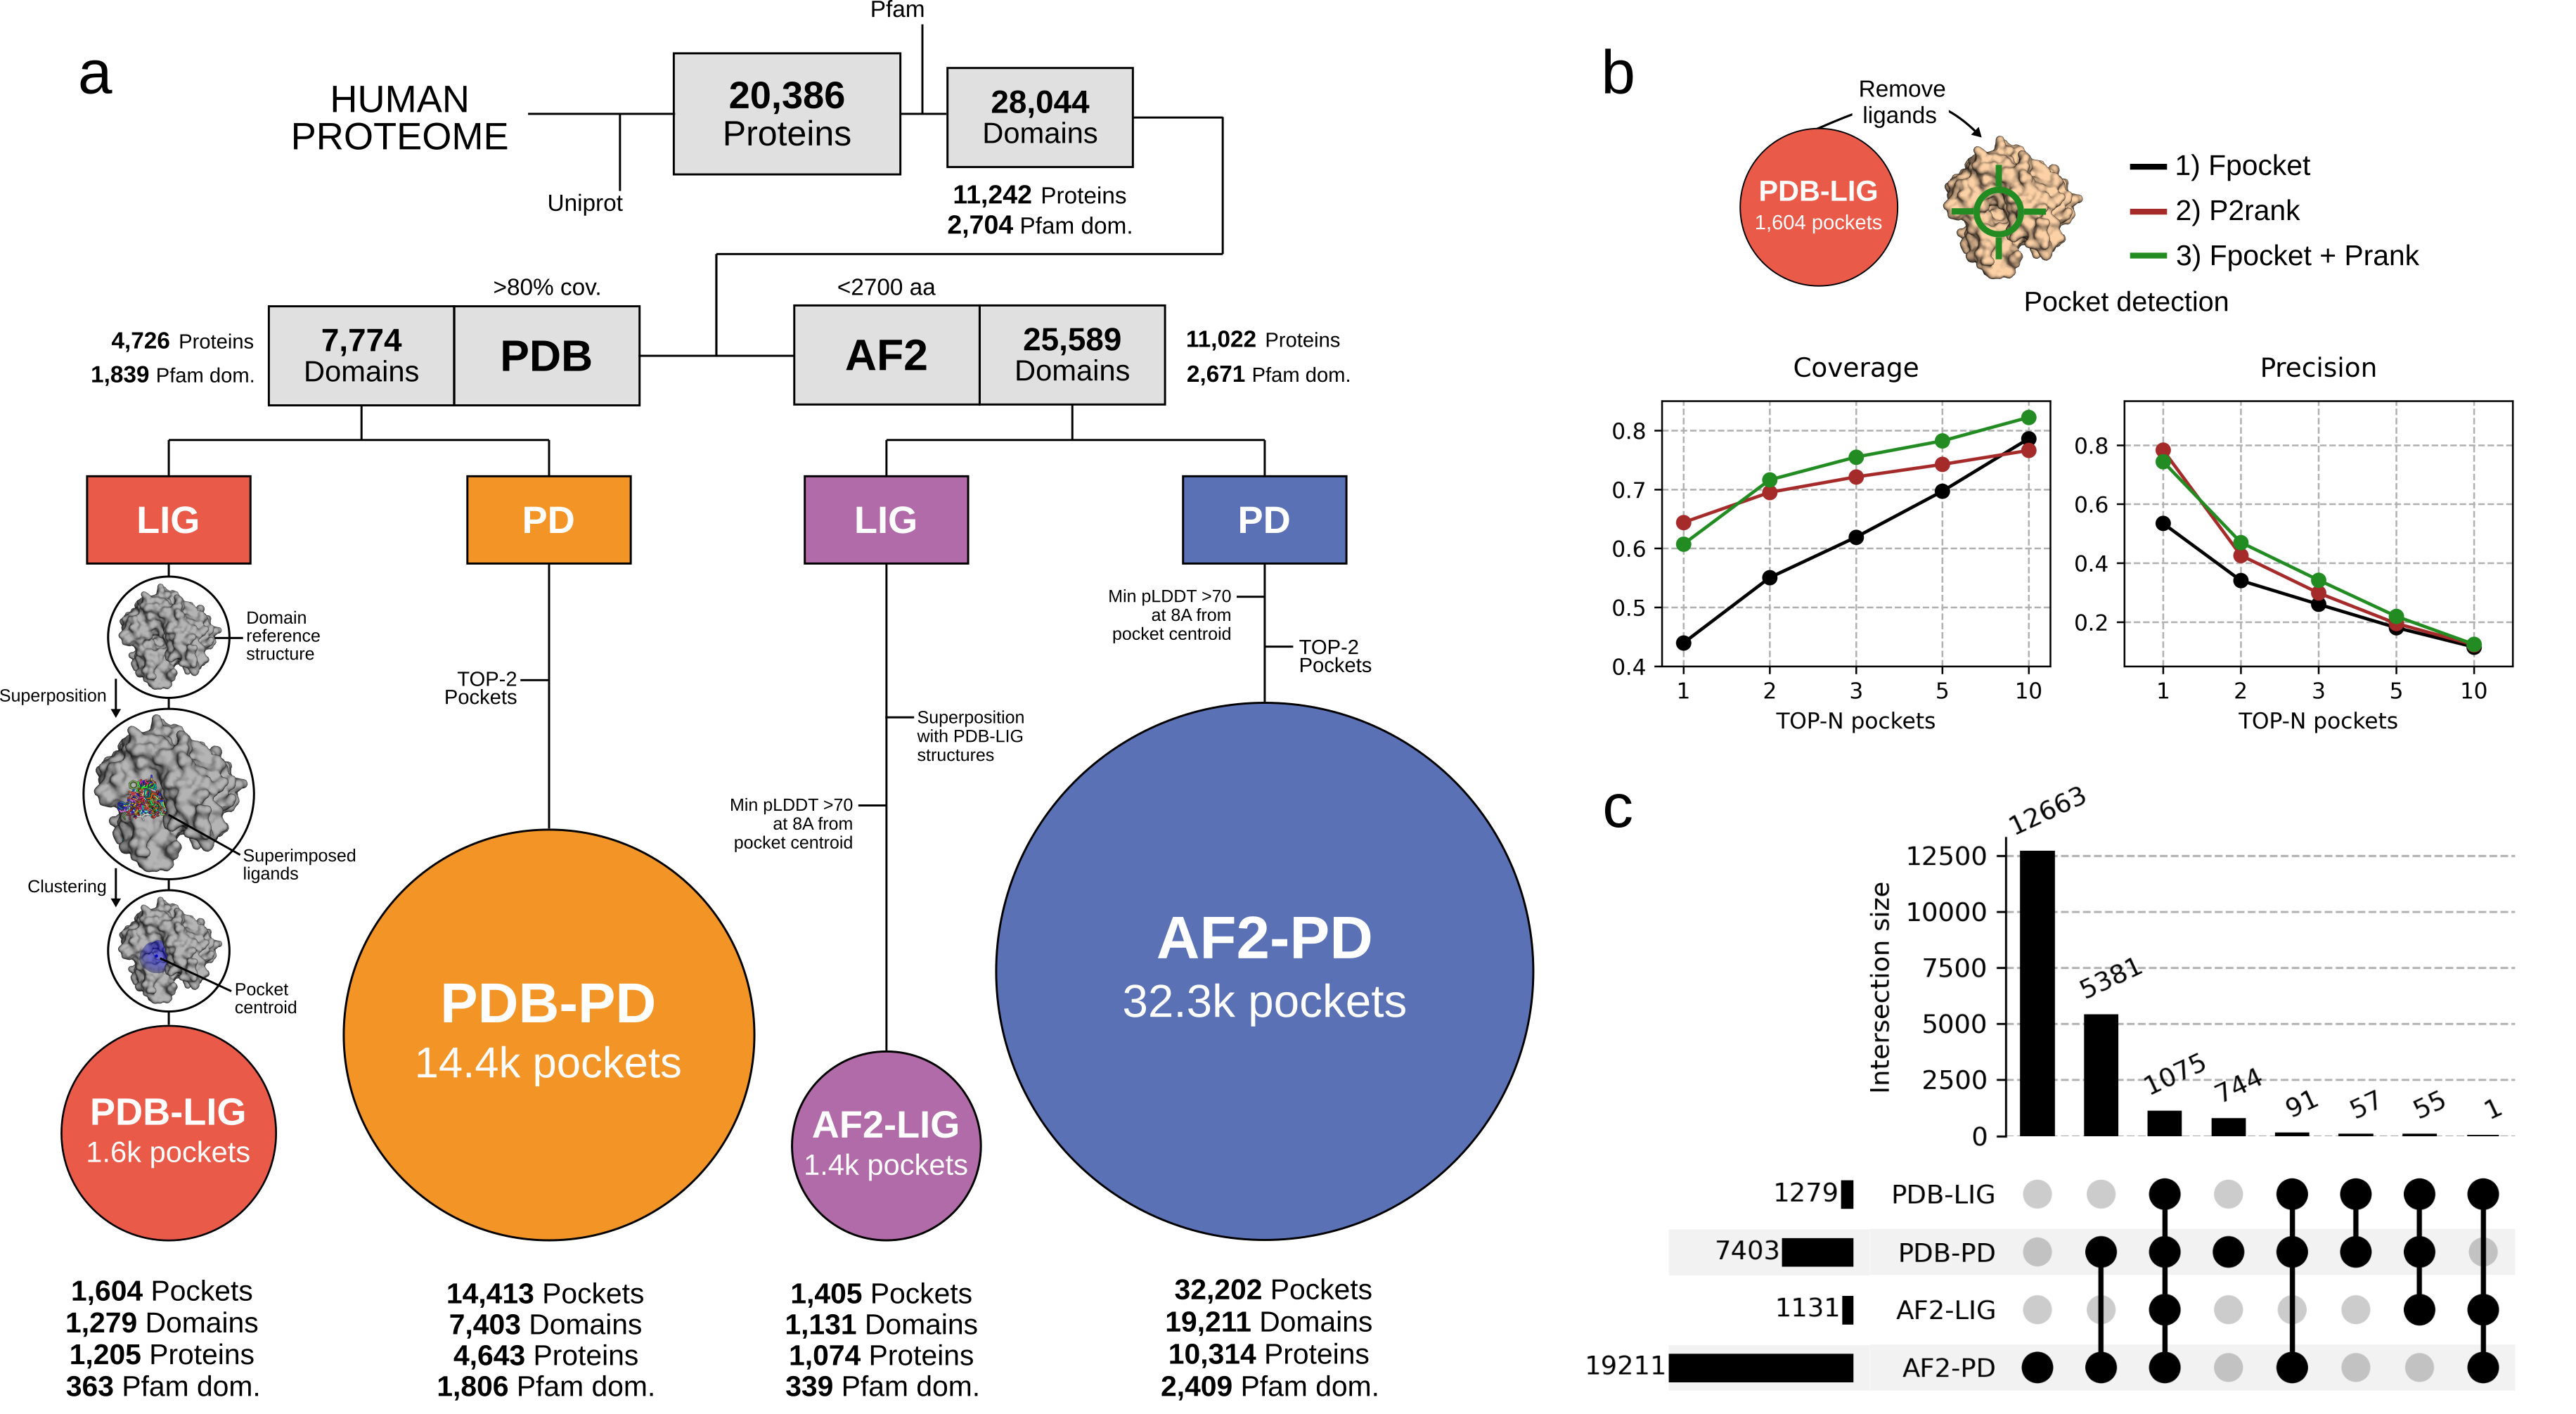
\includegraphics[width=\linewidth]{figures/PocketVec/Main/Fig2.png} 
  \caption{
    \textbf{Generating PocketVec descriptors for all druggable pockets within human protein domains.} 
    \textbf{a)} Computational pipeline to gather all available structural data for human druggable pockets included within protein Pfam domains. Starting from the complete human proteome as per Uniprot, we first identified Pfam domains in experimentally determined structures (PDB) and AF2 predicted models. For PDB structures, we identified pockets in \textit{holo} domain structures based on the position of co-crystallized ligands (1,604 PDB-LIG pockets, red) and in \textit{apo} domain structures using pocket detection techniques (14,413 PDB-PD pockets, orange). We defined ligand-based pockets on AF2 structures (1,405 AF2-LIG pockets, purple) by directly superimposing the location of PDB-LIG pockets, and pockets were also predicted in AF2 models by means of pocket detection algorithms (32,202 AF2-PD pockets, blue).  For additional details about the pipeline, please consult the text and the \hyperref[PocketVec_Methods]{Methods} section.
    \textbf{b)} Benchmark of 3 distinct pocket detection strategies: Fpocket (black), P2rank (brown) and the combination of Fpocket and Prank (green). First, we removed bound ligands from reference PDB structures (PDB-LIG) and we then assessed the performance of the mentioned strategies to detect pockets in ligand-free structures. The plots below represent the evolution of Coverage (proportion of real pockets that are actually detected) and Precision (proportion of detected pockets that are actually real -have a crystallized ligand on PDB-LIG) in terms of the number of best-scoring detected pockets per domain that are considered (1, 2, 3, 5 and 10).
    \textbf{c)} UpSet plot representing the intersecting number of domains among pocket sets (1,279 domains in PDB-LIG, 7,403 domains in PDB-PD, 1,131 domains in AF2-LIG and 19,211 domains in AF2-PD).
  }
  \label{PocketVec_Fig2}
\end{figure}


In brief, we first retrieved all 20,386 human proteins in UniProt\cite{the_uniprot_consortium_uniprot_2023}. To avoid working with unstructured or very flexible regions, difficult to model and unlikely to contain druggable pockets, we only kept those protein sequences within autonomous structural units (i.e. domains), as defined in Pfam\cite{mistry_pfam_2021}. Overall, we kept 28,044 domains (2,704 unique Pfam domains) in 11,242 human proteins (Fig \ref{PocketVec_FigS15}). The next step was to structurally annotate these domains, for which we used two different strategies. On the one hand, we looked for experimentally determined structures searching the PDB\cite{goodsell_rcsb_2020}, identifying at least one PDB structure for 7,774 domains (1,839 unique Pfam domains in 4,726 proteins). Additionally, we downloaded all human predicted protein structures from AlphaFold DB, obtaining structural models for 25,589 domains (2,671 unique Pfam domains in 11,022 proteins). There is an ongoing debate on the use of AF2 models for docking experiments, and whether such models should be refined using e.g. molecular dynamics simulations. However, most studies suggest that the accuracy of AF2 models in docking experiments is comparable to experimentally determined \textit{apo} structures (i.e. without a ligand bound)\cite{zhang_benchmarking_2023, holcomb_evaluation_2023, scardino_how_2023}. Indeed, it has been recently shown that the experimental validation rates of small molecule docking are indistinguishable when PDB structures or AF2 models are used\cite{lyu_alphafold2_2023}.

Next, for each domain, we identified the potentially druggable pockets, also using two different strategies. In the first one, that we termed \textit{ligand-based} pocket definition, we searched for small molecules co-crystallized together with the protein domain, and defined druggable pockets as those having bound compounds (HET PDB codes) fulfilling the following criteria: i) being annotated as such in PDBSUM data, ii) not being one of the 20 naturally occurring amino acids, iii) having more than 6 carbon atoms, to filter out solvent molecules and crystallography-related species and iv) having solvent accessibility ≤0.4 or buriedness ≥15 (\hyperref[PocketVec_Methods]{Methods}). In total, we found at least one PDB structure containing small molecules for 1,279 domains (363 unique Pfam domains in 1,205 proteins). For 503 of these, we only found a single ligand fulfilling our criteria, whereas for 254 of them we could find 10 or more ligands (Fig \ref{PocketVec_FigS16}). Then, to compile the list of unique ligand-defined pockets, we chose a reference PDB structure for each protein domain, and superimposed all domain structures with the corresponding bound ligands onto the reference. We then used a single-linkage clustering strategy to merge into a single pocket all those ligands whose centroids were at a distance ≤5Å while maintaining the maximum distance between the global centroid of the cluster and the centroids of the individual compounds ≤18Å. We considered the final global cluster centroids as the pocket centroids. Overall, we found 1,604 ligand-defined pockets in 1,279 protein domains (363 unique Pfam domains in 1,205 proteins). We named this set of pockets \textbf{PDB-LIG}. To apply the same criteria to those structures modeled with AF2, for each domain, we superimposed the reference PDB structure onto the AF2 model, and transferred the location of the identified PDB-LIG pockets accordingly. We only considered those pockets having a pLDDT value >70 for all residues at a distance ≤8Å from the pocket centroid. In total, we identified 1,405 pockets in 1,131 domains (339 unique Pfam domains in 1,074 proteins), and named this set \textbf{AF2-LIG}. As a complementary strategy, and to increase the overall coverage of the human pocketome, we attempted a de novo identification of druggable pockets. To find the most accurate strategy to predict druggable pockets, we assessed the accuracy of different methods at identifying the PDB-LIG pockets defined above. In brief, we first removed bound ligands from reference \textit{holo} structures and used Fpocket\cite{le_guilloux_fpocket_2009} and P2rank\cite{krivak_p2rank_2018}, to detect pockets in ligand-free domain structures (\hyperref[PocketVec_Methods]{Methods}). Our benchmark showed that the best strategy to detect binding sites in ligand-free structures was the combination of Fpocket, for pocket detection, and Prank to score them. Using this combination, and considering the top-2 best scored pockets for each domain, we were able to detect 72\% of the real pockets while 47\% of detected pockets were indeed real (Fig \ref{PocketVec_Fig2}b, coverage and precision, respectively). Thus, for each domain, we ran Fpocket on the PDB reference structure to identify potential pockets, we ranked them by means of Prank, and we kept the top-2 ranked pockets per domain. Overall, this accounted for a total of 14,413 predicted pockets in 7,403 domains (1,806 unique Pfam domains in 4,643 proteins). We named this set \textbf{PDB-PD}. We then used the same strategy and criteria as before to detect pockets onto the predicted AF2 domain models, annotating a total of 32,202 pockets in 19,211 domains (2,409 unique Pfam domains in 10,314 proteins). We named this set \textbf{AF2-PD}.



%%%%%%%%%%%%%%%%%%%%%%%%%%%%%%%%%%%%%%%%%%%%%%%%%%%%%%%%%%%%%%%%
%%% Robustness in the detection of druggable pockets
%%%%%%%%%%%%%%%%%%%%%%%%%%%%%%%%%%%%%%%%%%%%%%%%%%%%%%%%%%%%%%%%

\phantomsection
\subsubsection{Robustness in the detection of druggable pockets}
\label{PocketVec_ResultsAndDiscussion_Robustness_Detection}

Globally, using the different strategies to structurally annotate human protein domains and to identify validated and potential druggable pockets, we compiled 1,604 PDB-LIG, 1,405 AF2-LIG, 14,413 PDB-PD and 32,202 AF2-PD druggable pockets, in 20,067 domains (Fig \ref{PocketVec_Fig2}a and Fig \ref{PocketVec_Fig2}c). The significant added value of \textit{de novo} methodologies is very apparent. Indeed, for 18,788 domains (93.6\%), all pockets were identified only with pocket detection strategies and, among these, 12,663 domains (63.1\%) exclusively featured pockets on AF2 models (Fig \ref{PocketVec_Fig2}c).

Interestingly, when we assessed the methodological robustness of pocket predictions using a subset of 1,000 PDB-PD domains, we observed that results slightly differed after translating and rotating structures. This effect was observed for both PDB and AF2 structures in a consistent manner: only \textasciitilde85\% and \textasciitilde86\% of detected pockets were evenly identified after rotation and translation, respectively (top-2 pockets, Fig \ref{PocketVec_FigS17}a). However, in the pockets identified regardless of variations in the initial structures, the scoring was very consistent both in PDB structures and AF2 models (Pearson CC \textasciitilde0.98). We also evaluated the coherence between pockets detected in PDB and AF2 structures, finding that only \textasciitilde59\% and \textasciitilde49\% of detected pockets were evenly identified in PDB and AF2 structures with respect to a reference PDB structure. However, as when comparing discrepancies due to different initial orientations, in the pockets identified both in PDB and AF2 structures the scoring was quite robust, with Pearson CC of \textasciitilde0.88 and \textasciitilde0.62 for PDB and AF2 models, respectively (Fig \ref{PocketVec_FigS17}b). 

Additionally, we also explored potential differences in the physicochemical properties between the real (ligand-defined) and predicted (detected) pockets, comparing their volumes and buriedness values (see \hyperref[PocketVec_Methods]{Methods}). In this case, as the only remarkable difference, we found that real pockets identified from bound ligands tended to be smaller than those predicted in the PD framework, with average volumes of \textasciitilde3,000 Å3 and \textasciitilde3,800 Å3 for LIG and PD pockets, respectively (Fig \ref{PocketVec_Fig3}a). As expected, we reached the same conclusion with buriedness values (Fig \ref{PocketVec_FigS18}), since pocket volume and buriedness were indeed negatively correlated (Fig \ref{PocketVec_FigS19}).

Altogether, these results underscore some limitations in the pocket detection strategy, revealing slight variations due to the orientation of the initial structures, a stronger dependence on structural variability and the production of predicted pockets whose physicochemical properties (e.g. volume) diverge from known pockets. 


%%%%%%%%%%%%%%%%
%%% FIGURE 3 %%%
%%%%%%%%%%%%%%%%

\begin{figure}[htbp]
  \centering
  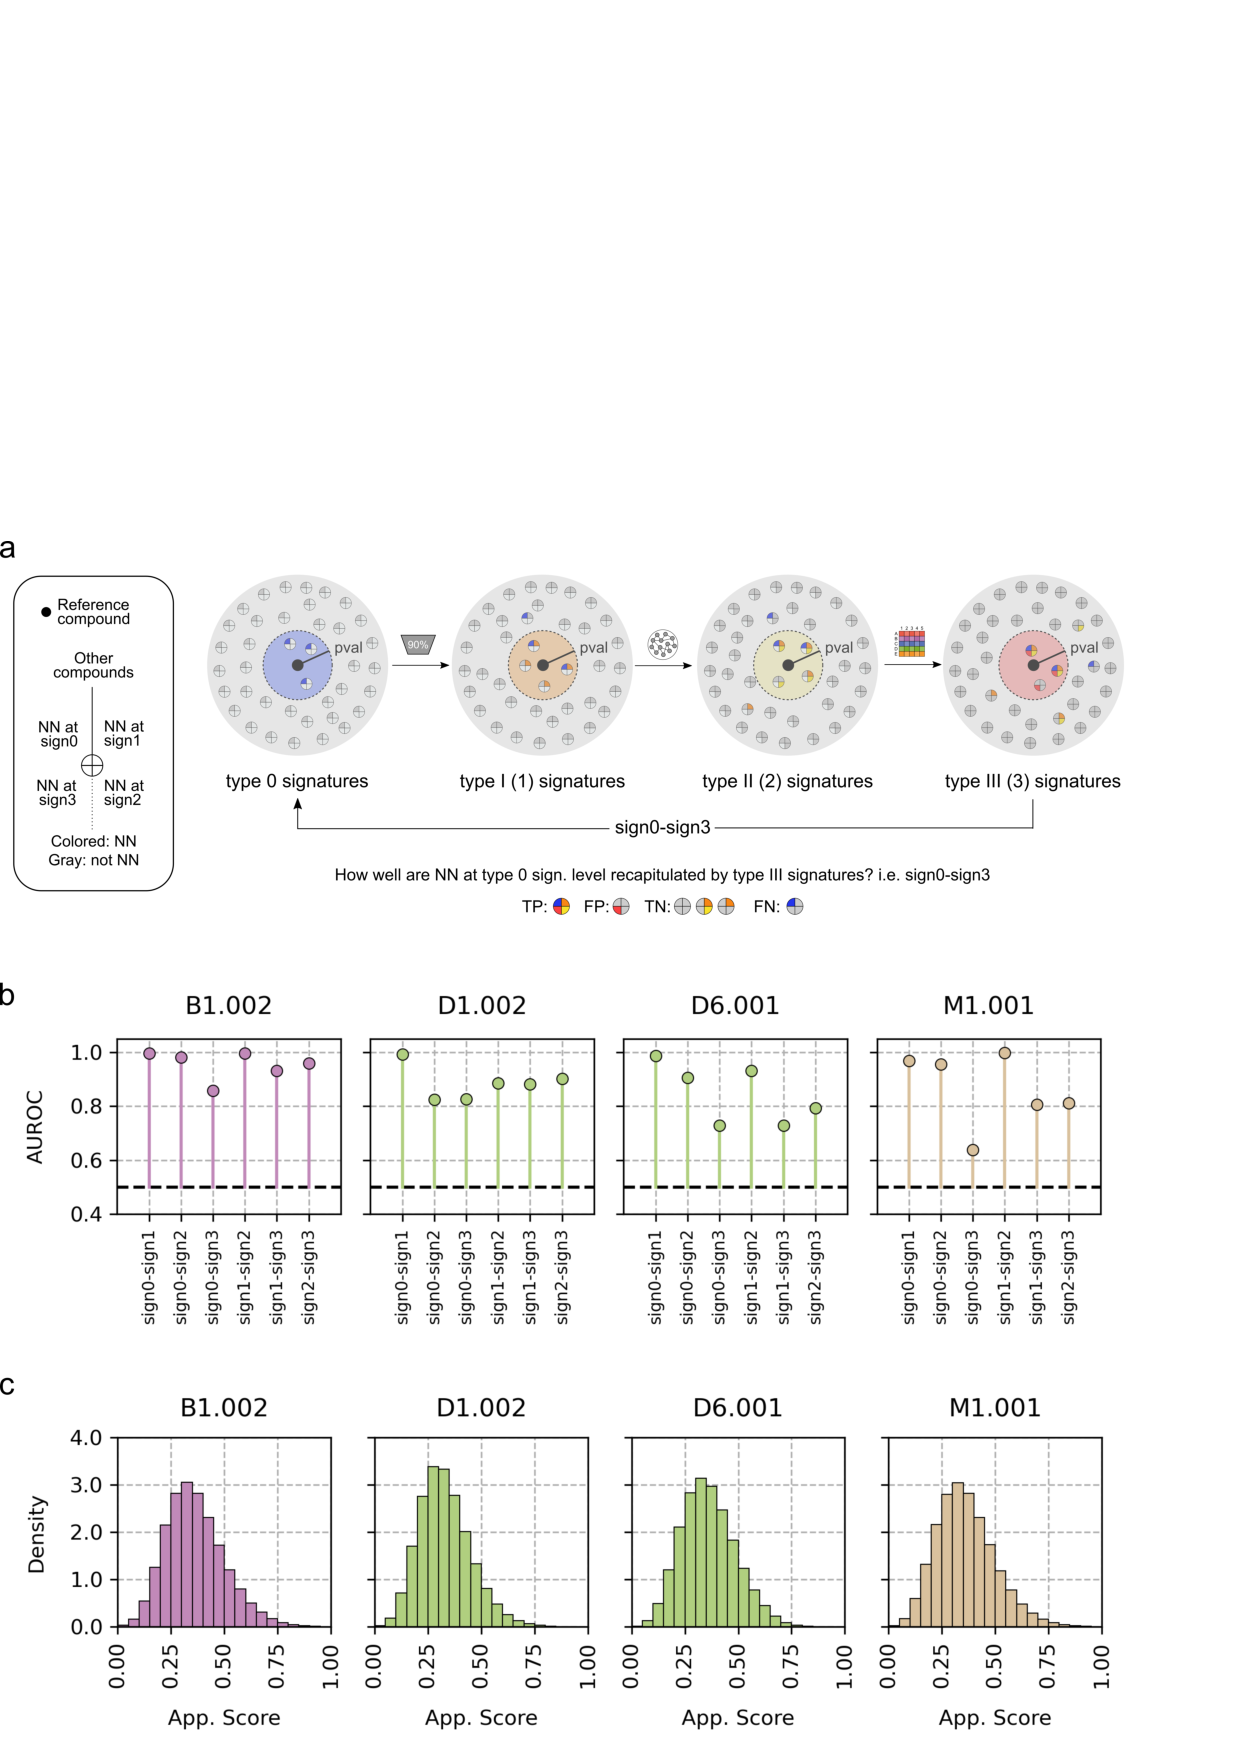
\includegraphics[width=\linewidth]{figures/PocketVec/Main/Fig3.png}
  \caption{
    \textbf{Characterization of human druggable pockets using PocketVec descriptors.} 
    \textbf{a)} Distribution of volumes (x-axis, x10³ A³) for each pocket set: PDB-LIG (1,604 pockets, red), PDB-PD (14,413 pockets, orange), AF2-LIG (1,405 pockets, purple) and AF2-PD (32,302 pockets, blue). All distributions are normalized (density, y-axis). The average volumes are 2992.88 A³, 3764.1 A³, 2940.47 A³ and 3972.66 A³, respectively. Pocket volumes were directly calculated using the rDock\cite{ruiz-carmona_rdock_2014} CAVITY functionality. 
    \textbf{b)} Correlation between average docking rankings among all pocket sets. For each pocket set, a 128-length array containing the average docking ranking for each lead-like molecule was calculated, and these arrays were compared among pocket sets by means of the Pearson’s Correlation Coefficient. All p-values (10) are <10\textsuperscript{-25}. 
    \textbf{c)} For each pocket set, proportion of PocketVec descriptors (\%, y-axis) having less than N (x-axis) outlier molecules (i.e. molecules with positive docking scores, please see \hyperref[PocketVec_Methods]{Methods}).
    \textbf{d)} Proportion of originally dissimilar pocket pairs (y-axis, distances >threshold) classified as similar (distances <threshold) due to the artificial insertion of a growing number of outlier values (x-axis) at different distance thresholds. To run the analysis, 100,000 PocketVec distances were randomly sampled (x10 times) from PDB-LIG. Solid lines represent average results and shadowed areas correspond to minimum and maximum proportions among samples. Results did not change among pocket sets (Fig \ref{PocketVec_FigS23}).
    \textbf{e)} tSNE (t-distributed Stochastic Neighbor Embedding) representation of all PocketVec descriptors within each pocket set (PDB-LIG, PDB-PD, AF2-LIG, AF2-PD). Each pocket is represented by a single point, which is colored and sized by 2D density within the pocket set. Gray dots correspond to the background space: all PocketVec descriptors are considered at once, and are also colored and sized by 2D density.
    \textbf{f)} Distributions (density, y-axis) of maximum Tanimoto Similarity among bound ligands (x-axis, bin width: 0.02) grouped by PocketVec distance ranges (0-0.10, 0.10-0.17 and 0.17-0.4). The number of pocket pairs per PocketVec distance range is specified in parenthesis.
    \textbf{g)} Distributions (density, y-axis) of PocketVec cosine distances (x-axis) grouped by the maximum Tanimoto Similarity among bound ligands (0-0.5, 0.5-0.8, 0.8-1 and 1). The number of pocket pairs per maximum Tanimoto Similarity range is specified in parenthesis.
    \textbf{h)} Distributions (density, y-axis) of PocketVec cosine distances (x-axis) grouped by the number of shared ligands between pockets (0, 1, 2 and 3 or more). The number of pocket pairs per number of shared ligands is specified in parenthesis.
  }
  \label{PocketVec_Fig3}
\end{figure}


%%%%%%%%%%%%%%%%%%%%%%%%%%%%%%%%%%%%%%%%%%%%%%%%%%%%%%%%%%%%%%%%
%%% Systematic generation of PocketVec descriptors
%%%%%%%%%%%%%%%%%%%%%%%%%%%%%%%%%%%%%%%%%%%%%%%%%%%%%%%%%%%%%%%%

\phantomsection
\subsubsection{Systematic generation of PocketVec descriptors}
\label{PocketVec_ResultsAndDiscussion_Systematic_generation_of_PocketVec_descriptors}


Once we had identified human druggable pockets with four different approaches, we systematically generated PocketVec descriptors for all of them, using the strategy described above (Fig \ref{PocketVec_Fig1}a). The high number of pockets explored enabled an exhaustive analysis of potential dependencies between the lead-like molecules used to build the descriptors and the characterization of druggable pockets. Reassuringly, we did not find any correlation between docking rankings and molecular properties of docked compounds (e.g. molecular weight or number of heavy atoms, Fig \ref{PocketVec_FigS20} and Fig \ref{PocketVec_FigS21}, respectively). On the contrary, we observed that most molecules exhibited a complete range of rankings (from 1 to 128), although the ranking distributions showed that some molecules tended to bind with good scores in many pockets while others were mostly downranked (Fig \ref{PocketVec_FigS22}). Indeed, this tendency was observed in all pocket definition strategies, and we found significant correlations between the average docking rankings for docked lead-like molecules among different pocket sets (Fig \ref{PocketVec_Fig3}b). Such correlations showed a perfect agreement between PocketVec descriptors generated through PDB and AF2 structures, but exposed slight differences between LIG and PD results (Fig \ref{PocketVec_Fig3}b, Pearson’s CC <0.88). In line with this, we found that 88.0\% and 86.8\% of the PocketVec descriptors generated for PDB-LIG and AF2-LIG, respectively, showed no lead-like molecules with positive docking scores (i.e. outlier molecules not fitting in the pocket, see \hyperref[PocketVec_Methods]{Methods}), while the fraction was considerably higher in PDB-PD and AF2-PD sets, with 97.0\% and 98.1\% of the descriptors, respectively (Fig \ref{PocketVec_Fig3}c). This result was consistent with the differences observed in pocket volumes (Fig \ref{PocketVec_Fig3}a). Reassuringly, we found that smaller pockets (<3,000ų) tended to be more prone to exhibit outlier molecules than bigger pockets (Fisher exact test, OR >70 and p-value <10\textsuperscript{-45} for all pocket sets).


To assess if outlier compounds could have a significant effect in the generation of poor PocketVec descriptors, we randomly inserted outlier values in the descriptors and computed the fraction of originally dissimilar pocket pairs (PocketVec distance >0.17) that were incorrectly labeled as similar (distance <0.17) due to an increasing number of outlier values. We observed that the insertion of up to 80 outlier molecules (out of 128) did not significantly compromise PocketVec descriptors, leading to only \textasciitilde0.039\% of false positives (Fig \ref{PocketVec_Fig3}d and Fig \ref{PocketVec_FigS23}). In front of this strong robustness of the descriptors, in further analyses, we only discarded those very few PocketVec descriptors with more than 80 outlier molecules (10, 45, 15 and 43 descriptors from the PDB-LIG, PDB-PD, AF2-LIG and AF2-PD sets, respectively). 



%%%%%%%%%%%%%%%%%%%%%%%%%%%%%%%%%%%%%%%%%%%%%%%%%%%%%%%%%%%%%%%%
%%% Influence of protein flexibility on PocketVec descriptors
%%%%%%%%%%%%%%%%%%%%%%%%%%%%%%%%%%%%%%%%%%%%%%%%%%%%%%%%%%%%%%%%

\phantomsection
\subsubsection{Influence of protein flexibility on PocketVec descriptors}
\label{PocketVec_ResultsAndDiscussion_Influence_of_protein_flexibility}

Proteins are dynamic entities that may adopt various 3D conformations depending on multiple environmental factors (e.g. the presence of a ligand), as well as exhibiting a certain degree of flexibility in their side chains. Indeed, a single X-ray structure often does not represent the complete structural behavior of a protein, and we thus do not expect a single PocketVec descriptor to be a global representation of a pocket but instead a snapshot for each particular structure. To some extent, the ProSPECCTs benchmark set already assesses the sensitivity of PocketVec descriptors to the binding site definition (i.e. same pocket occupied by distinct ligands, P1 and P1.2) and the impact of protein flexibility (i.e. NMR-resolved structures, P2). In this context, we observed that, as expected, the variability among PocketVec descriptors from the same pocket was lower enough to be clearly distinguished from random pairs of pockets (Fig \ref{PocketVec_Fig1}d, AUROCs of 0.97, 1.00 and 0.96 for ProSPECCTs P1, P1.2 and P2, respectively). Besides, a 2D tSNE representation of PocketVec descriptors derived from the 326 structures in P1 showed a clustering pattern consistent with the 12 pockets represented (Fig \ref{PocketVec_Fig4}a). Interestingly, we observed that one of the structures (3UAB\_B) of Poly-ADP polymerase tankyrase-2 (Q9H2K2) significantly deviated from the rest of the descriptors from the same pocket (protein) in the tSNE representation (black dots), and a visual inspection of its structure showed significant conformational changes in the side chains conforming the binding pocket with respect to the other ones (Fig \ref{PocketVec_Fig4}b), which translated into a higher PocketVec distance (>0.17) with the rest of the descriptors of the same pocket. In any case and, as briefly mentioned above, PocketVec descriptors for holo structures of the same pocket (ProSSPECTs P1 similar pairs) were fairly similar, with almost 80\% of the pairs showing distances <0.17, while only 1,2\% of the pairs showed distances <0.17 for dissimilar pocket pairs. When comparing holo structures to the corresponding apo structures or AF2 models of the same pocket, we found that the PocketVec descriptors showed higher variability than within \textit{holo} structures, reflecting pocket structural heterogeneity (Fig \ref{PocketVec_FigS24}). However, the distributions of distances comparing \textit{holo} with \textbf{apo} or AF2 structures were very similar, with 51\% and 55\% of pairs pairs below the 0.17 threshold, respectively. To further complement this result, we performed an exhaustive evaluation of the behavior of PocketVec descriptors upon protein flexibility and conformational changes. In short, we kept those pockets from the PDB-LIG set for which we had enough \textit{holo} and \textit{apo} PDB structures available (≥10, see \hyperref[PocketVec_Methods]{Methods}) as well as a confident AF2 model, and generated PocketVec descriptors for all their structures. Overall, we collected 903 PocketVec descriptors corresponding to 43 unique pockets (10 holo structures, 10 apo structures and 1 AF2 model each). We then computed PocketVec distances between same-pocket holo PDB structures (LIG-LIG), same-pocket holo and apo PDB structures (LIG-PD), same-pocket apo PDB structures (PD-PD), same-pocket holo PDB and AF2 structures (LIG-AF2) and, finally, same-pocket apo PDB and AF2 structures (PD-AF2). Additionally, we compared holo (PDB), apo (PDB) and AF2 structures against our 4 sets of precompiled PocketVec descriptors (i.e. PDB-LIG, PDB-PD, AF2-LIG and AF2-PD) in order to contextualize the results with background distance distributions (Fig \ref{PocketVec_Fig4}c). We observed that PocketVec descriptors derived from holo PDB structures were rather robust and clearly distinguishable from random pocket pairs (LIG-LIG, AUROC of 0.90 against background distance distributions), in perfect agreement with the results obtained in ProSPECCTs P1 and P1.2. When we compared descriptors derived from holo and apo PDB structures, as expected, the intrinsic and increased variability of ligand-free structures was reflected in the PocketVec distances, which affected the ability to recapitulate pocket structures from the same protein (LIG-PD, AUROC of 0.77; PD-PD, AUROC of 0.80). Finally, we also observed that descriptors derived from holo structures tended to be more similar to those derived from AF2 models than to those from apo PDB structures (LIG-AF2, AUROC of 0.82). This observation aligns with several studies stating that AF2-predicted structures are comparable to the apo conformations and, perhaps, a bit closer to the holo conformations due to the nature of the training data (which includes both holo and apo structures)\cite{zhang_benchmarking_2023}.


Additionally, we sampled MD trajectories for 192 pockets from the PDB-LIG and PDB-PD sets, considering 10 conformations per pocket, and then, for each pocket, we calculated all pairwise distances among their PocketVec descriptors (see Online Methods). As in the previous exercise, we also compared the obtained PocketVec descriptors with a random sample of precomputed descriptors from the PDB-LIG, PDB-PD, AF2-LIG and AF2-PD sets (Fig \ref{PocketVec_Fig4}d). Overall, we observed a similar trend than when comparing \textit{apo} PDB structures: PocketVec descriptors showed variations responding to the flexibility of the proteins, while still recognizing different conformations from the same pocket (AUROC of 0.78). Finally, we analyzed the correlation between PocketVec distance among MD frames and the all-atom RMSD (excluding hydrogen atoms) considering both complete structures and only pocket residues (at <8Å from the pocket centroid in any of the MD used frames). We found a weak correlation (Fig \ref{PocketVec_Fig4}e; Pearson CC 0.39) with the full structure RMSD that increased (Fig \ref{PocketVec_Fig4}f; Pearson CC 0.49) when exclusively considering pocket residues. 

The presence of metal atoms is often required for many pockets to perform its native function (e.g. to act as catalytic centers or to stabilize protein structures). However, our study does not explicitly consider the presence of other compounds such as cofactors or metal atoms which, despite the limitations, it enables a fair and analogous characterization with different protein structures and pocket identification strategies where bound metal atoms are not available (e.g. PDB vs AF2 or LIG vs PD). Thus, finally, we also assessed the ability of our precomputed PocketVec descriptors to identify pocket similarities among metal-binding proteins. For this, after collecting all PDB-LIG and PDB-PD pockets with bound metal atoms, we compared the derived PocketVec descriptors with and without the metal atoms (\hyperref[PocketVec_Methods]{Methods}). We observed that, although descriptors were obviously not identical, the vast majority of the identified metal-binding pockets had similar PocketVec descriptors with and without the explicit presence of the metal atoms (Mann-Whitney p-value <10\textsuperscript{-100}; Fig \ref{PocketVec_FigS25}). 

Overall, these results illustrate the capacity of PocketVec descriptors to capture pocket flexibility and protein conformational changes, revealing their sensitivity to changes in the pocket shapes as well as their feasibility of use with \textit{holo} and \textit{apo} PDB structures (including metal-binding proteins) and AF2 predicted models. 


%%%%%%%%%%%%%%%%
%%% FIGURE 4 %%%
%%%%%%%%%%%%%%%%


\begin{figure}[H]
  \centering
  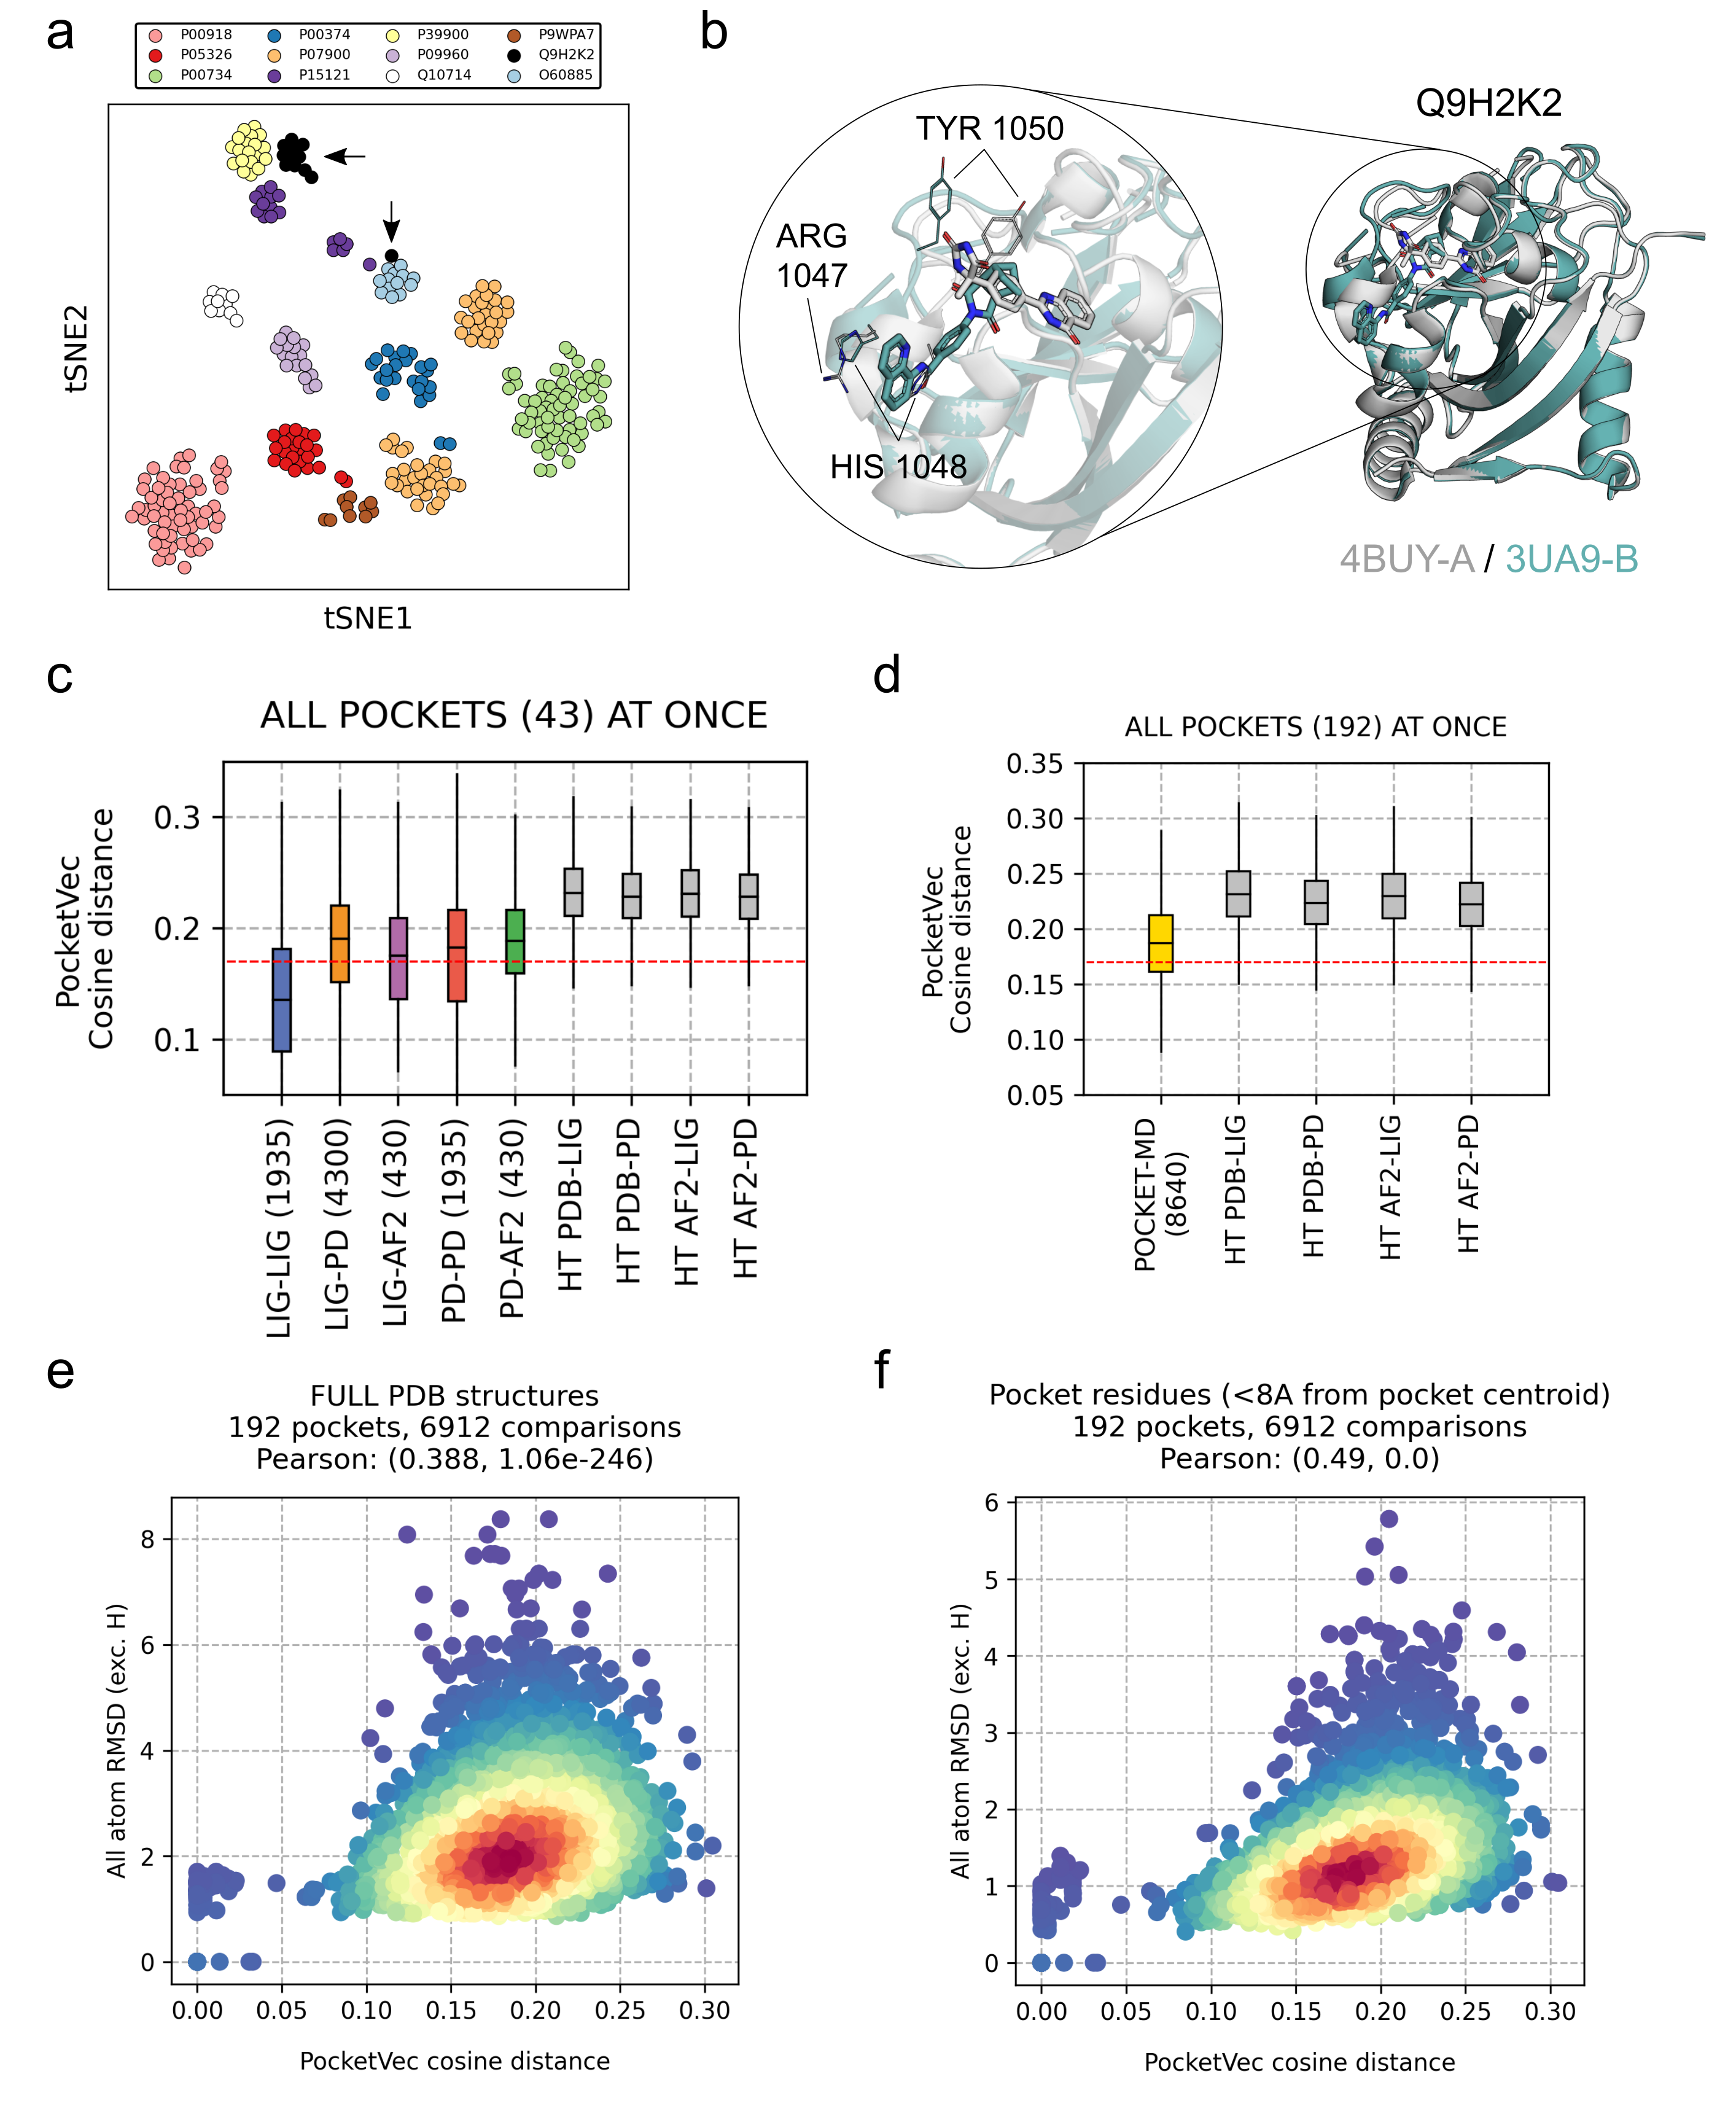
\includegraphics[width=\linewidth]{figures/PocketVec/Main/Fig4.png} 
  \caption{
    \textbf{Assessment of the effect of protein flexibility.} 
    \textbf{a)} 2D tSNE representation of 326 PocketVec descriptors representing the conformational ensemble of 12 pockets binding distinct ligands (ProSPECCTs P1). Black arrows indicate the Poly-ADP polymerase tankyrase-2 (Q9H2K2) structures.
    \textbf{b)} Structural superimposition of 4BUY\_A (white) against 3UA9\_B (teal) performed with TM-align\cite{zhang_tm-align_2005}.
    \textbf{c)} PocketVec descriptors’ variability caused by protein flexibility and conformational changes. Each boxplot indicates the distribution of PocketVec distances of the same pocket in i) holo PDB structures (LIG-LIG), ii) holo and apo PDB structures (LIG-PD), iii) holo PDB and AF2 structures (LIG-AF2), iv) apo PDB structures (PD-PD), v) apo PDB and AF2 structures (PD-AF2) and holo (LIG), apo (PD) and AF2 structures (AF2) against each of the 4 sets of PocketVec descriptors from our study (i.e. PDB-LIG, PDB-PD, AF2-LIG, AF2-PD). Boxplots indicate median (middle line), 25th, 75th percentile (box), and max and min value within the 1.5*25th and 1.5*75th percentile range (whiskers).
    \textbf{d)} PocketVec descriptors’ variability caused by protein flexibility and conformational changes among MD-derived structures. POCKET-MD represents the distances between same-pocket MD-derived PocketVec descriptors and all the other boxplots represent the distances between such MD-derived descriptors and each of the 4 sets already precomputed (i.e. PDB-LIG, PDB-PD, AF2-LIG, AF2-PD).
    \textbf{e)} Correlation between PocketVec cosine distance (x-axis) and all-atom (excluding hydrogens) RMSD for the full PDB structure and
    \textbf{f)} pocket residues only. The study involved 192 pockets (8 from PDB-LIG and 184 from PDB-PD) with MD-simulation data (3 frames per replica, 3 replicas). Both plots are colored by density (the redder the higher).
  }
  \label{PocketVec_Fig4}
\end{figure}


%%%%%%%%%%%%%%%%%%%%%%%%%%%%%%%%%%%%%%%%%%%%%%%%%%%%%%%%%%%%%%%%
%%% All-vs-all comparison of human druggable pockets
%%%%%%%%%%%%%%%%%%%%%%%%%%%%%%%%%%%%%%%%%%%%%%%%%%%%%%%%%%%%%%%%

\phantomsection
\subsubsection{All-vs-all comparison of human druggable pockets}
\label{PocketVec_ResultsAndDiscussion_All_vs_All_comparison_human_druggable_pockets}

The vector-like nature of PocketVec descriptors makes them perfectly suited for extremely fast comparisons by computing simple cosine distances, enabling comprehensive proteome-wide similarity searches. We first generated a t-distributed Stochastic Neighbor Embedding (t-SNE) representation for all PocketVec descriptors to facilitate a qualitative visualization of the characterized pocket space (Fig \ref{PocketVec_Fig3}e). This visualization underlined several interesting points, some of which have already been discussed in previous sections: (i) pockets defined by bound ligands (PDB-LIG and AF2-LIG) predominantly occupy well defined regions of the pocket space, (ii) pocket detection strategies (PDB-PD and AF2-PD) significantly contribute to expand the overall coverage of the human druggable pocket space, (iii) the use of AF2 models particularly bolsters this expansion. Perhaps more interestingly, the PDB-PD and AF2-PD maps highlight dense areas of the human pocket space for which we do not yet have any experimental structure with a bound chemical compound.

Then, we systematically evaluated the validity of the chemogenomic hypothesis behind the generation of PocketVec descriptors (i.e. similar pockets bind similar ligands). We compared all PDB-LIG pockets having PocketVec descriptors (1,594 pockets, \textasciitilde1.27M comparisons) on the basis of the maximum Tanimoto similarity among their bound ligands using ECFPs (2,048 bits and radius 2), and we grouped pocket pairs according to their cosine PocketVec distance (Fig \ref{PocketVec_Fig3}f). We found that, indeed, pocket pairs with small PocketVec distances (<0.10) typically showed higher maximum Tanimoto similarities (>0.85) among their ligands than pocket pairs with high PocketVec distance (>0.17, Fisher’s exact test OR >90 and p-value <10\textsuperscript{-300}), thus supporting our underlying hypothesis. However, the fact that similar pockets bind similar ligands does not necessarily imply that similar ligands bind similar pockets. Indeed, we observed that, in general, PocketVec distances did not decrease substantially when increasing the maximum Tanimoto similarity among bound ligands (Fig \ref{PocketVec_Fig3}g). The only exception was for almost identical ligands (Tanimoto similarities=1), which showed a very subtle deviation towards smaller PocketVec distances (AUROC 0.59, true positives having Max. Tanimoto Similarity=1, true negatives having Max. Tanimoto Similarity in the [0, 0.5) range), in line with the behavior observed in ProSPECCTs P5 (AUROC=0.64) and P5.2 (AUROC=0.62). While this may seem somewhat counterintuitive, it serves as evidence to decipher the quantification of pocket similarity using PocketVec descriptors. 

The fact that a single compound is consistently upranked for two pockets may indeed be a first evidence of pocket similarity but falls short to provide similar PocketVec descriptors if no other compound is ranked in a systematic manner. In practical terms, this translates into pockets that share a growing number of ligands being more likely to be similar from a PocketVec perspective, as highlighted by Shoichet and co-workers when they presented their similarity ensemble approach (SEA) to unveil protein remote relationships\cite{keiser_relating_2007}. Reassuringly, we found that pockets that shared ligands in the PDB-LIG set tended to be more similar (i.e. smaller PocketVec distances) than pockets sharing no ligands (Fig \ref{PocketVec_Fig3}h). However, the deviation towards smaller distances for pockets sharing a single ligand was subtle (AUROC = 0.58, true positives sharing 1 ligand and true negatives sharing no ligands), but when 3 or more ligands were shared between pockets, the effect was already notable (AUROC = 0.75, true positives sharing 3 or more ligands and true negatives sharing no ligands). We also found that only 2.1\% of pocket pairs sharing no ligands in the PDB-LIG set showed PocketVec distances <0.17, while this fraction increased to 26.1\% when 3 or more ligands were shared between pockets. However, it is obvious that the lack of shared co-crystallized compounds between two pockets does not necessarily mean that they might not have common ligands. To overcome the limitation of potentially missing ligands, we used a pure computational strategy: we computed docking scores for the 128 standard lead-like molecules (see \hyperref[PocketVec_MethDevAndImp]{Methodological development and implementation}) against all PDB-LIG defined pockets and labeled them as active (the top 1\% of docking scores) or inactive (Fig \ref{PocketVec_FigS26}a). We observed that the vast majority of the lead-like molecules (127 out of 128) were cataloged as active in, at least, one pocket (Fig \ref{PocketVec_FigS26}b), and almost 20,000 of the potential \textasciitilde1,29M PDB-LIG pocket pairs shared, at least, one active lead-like molecule (Fig \ref{PocketVec_FigS26}c). With this alternative approach, we confirmed the tendency observed using experimental data: the more shared ligands between pockets, the smaller their PocketVec distance (AUROC = 0.87 when comparing pockets sharing no ligands and those sharing 3 or more ligands; Fig \ref{PocketVec_FigS26}d).

Next, we explored the complementarity and added value of PocketVec descriptors with respect to more established strategies to compare protein families and druggable pockets, such as sequence and structure similarity. First, we sought to investigate the correlation between sequence, structure and PocketVec similarity (defined as 1-PocketVec distance) among pockets located in the same Pfam domains in the more comprehensive set of AF2-PD pockets (see \hyperref[PocketVec_Methods]{Methods}). As expected, we found that the higher the sequential and structural similarity between compared pockets (assessed by sequence identity and Cα RMSD, respectively), the more similar they were according to PocketVec descriptors (Pearson CC of 0.55 and -0.35, respectively, p-value<10\textsuperscript{-100} in both cases; Fig \ref{PocketVec_Fig5}a). Reassuringly, the observed correlations were also found when computed on AF2-LIG pockets (Pearson CC of 0.57 and -0.35 for sequence identity and Cα RMSD, respectively Fig \ref{PocketVec_FigS27}). However, there were indeed cases where the results did not align perfectly, underscoring the distinctive and complementary insights that PocketVec descriptors can provide beyond traditional sequential and structural analyses.

Additionally, we also ran an all-against-all pocket comparison within and across pocket sets (PDB-LIG, PDB-PD, AF2-LIG and AF2-PD), computing over 1.2 billion pocket comparisons. Interestingly, we found more than 3.5 million similar pockets in domains having low sequential and structural similarities (PocketVec distance <0.17; TM-score <0.35; Sequence identity <30\%). For instance, we found similar pockets (PocketVec distance: 0.14, both pockets in the PDB-LIG set) in the CPSase\_L\_D2 ATP-binding domain (PF02786) of the Carbamoyl-phosphate synthase (P31327, positions 1088-1291) and in the NDK domain of the Nucleoside diphosphate kinase 3 (Q13232, positions 22-156), although they shared a sequence identity of only 28\% and a poor structural similarity (TM-score=0.31, RMSD=4.3Å). Reassuringly, crystal structures confirmed that both pockets can bind ADP (PDB IDs: 5DOU and 1ZS6, respectively), which strengthened our observation that these pockets were indeed similar (Fig \ref{PocketVec_Fig5}b). The inventory of all similar pockets (PocketVec distance <0.17) together with structural and sequential comparisons at domain level are reported in our \hl{GitLab}. On the other hand, our analyses also revealed more than 29k pocket pairs (out of a subsample of 11.1 million pairs having PocketVec distance >0.20) that, despite being similar in terms of sequence and structure, showed quite dissimilar pockets (PocketVec distance >0.20; TM-score >0.50; Sequence identity >40\%). As an illustrative example, we identified different druggable pockets (PocketVec distance: 0.21, both pockets in the AF2-PD set) in the NIPSNAP domain (PF07978) of the Protein NipSnap homolog 3B (Q9BS92, positions 146-245) and in the NIPSNAP domain (PF07978) of the Protein NipSnap homolog 3A (Q9UFN0, positions 146-245), although these domains had a sequence identity of 93\% and also a very high level of structural similarity (Fig \ref{PocketVec_Fig5}c, TM-score=0.98 and RMSD=0.4Å).

%%%%%%%%%%%%%%%%
%%% FIGURE 5 %%%
%%%%%%%%%%%%%%%%

\begin{figure}[H]
  \centering
  \includegraphics[width=\linewidth]{figures/PocketVec/Main/Fig5.png} 
  \caption{
    \textbf{Using PocketVec descriptors to assess proteome-wide pocket similarity: achieving otherwise unattainable insights.} 
    \textbf{a)} Correlation between PocketVec similarity (x-axis, defined as 1-PocketVec distance), structural similarity (y-axis, Cα RMSD) and sequence identity (color) among pockets located at the same Pfam domains (max. 10) in the AF2-PD pocket set. Pearson CC between PocketVec similarity and sequence identity: 0.55 (p-value\textasciitilde0). Pearson CC between PocketVec similarity and RMSD: -0.35 (p-value\textasciitilde0).
    \textbf{b)} Similar pockets found in dissimilar domains. Pockets were found in the CPSase\_L\_D2 ATP-binding domain (PF02786, top structure, wheat color) of the Carbamoyl-phosphate synthase (P31327, positions 1088-1291. PDB ID: 5DOU) and in the NDK domain (PF00334, bottom structure, pale green color) of the Nucleoside diphosphate kinase 3 (Q13232, positions 22-156. PDB ID: 1ZS6). Pockets (both in the PDB-LIG set) have a PocketVec distance of 0.14 (below the established threshold of 0.17, please see \hyperref[PocketVec_ResultsAndDiscussion_PocketVec_performance_on_the_ProSPECCTs_benchmark]{PocketVec performance on the ProSPECCTs benchmark sets}) although domains share a sequence identity of only 28\% and a poor structural similarity (TM-score=0.31, RMSD=4.3Å).
    \textbf{c)} Dissimilar pockets found in similar domains. Pockets were found in the NIPSNAP domain (PF07978) of the Protein NipSnap homolog 3B (Q9BS92, positions 146-245, AF2 model, pink residues) and in the NIPSNAP domain (PF07978) of the Protein NipSnap homolog 3A (Q9UFN0, positions 146-245, AF2 model, green residues). The former is used as the reference structure (gray cartoon). Pockets (both in the AF2-PD set) have a PocketVec distance of 0.21 (above the established threshold of 0.17, please see \hyperref[PocketVec_ResultsAndDiscussion_PocketVec_performance_on_the_ProSPECCTs_benchmark]{PocketVec performance on the ProSPECCTs benchmark sets}) although domains have a sequence identity of 93\% and also a very high level of structural similarity (TM-score=0.98 and RMSD=0.4Å).
  }
  \label{PocketVec_Fig5}
\end{figure}




%%%%%%%%%%%%%%%%%%%%%%%%%%%%%%%%%%%%%%%%%%%%%%%%%%%%%%%%%%%%%%%%
%%% Relationship between PocketVec similarity and experimentally determined compound-target pairs
%%%%%%%%%%%%%%%%%%%%%%%%%%%%%%%%%%%%%%%%%%%%%%%%%%%%%%%%%%%%%%%%

\phantomsection
\subsubsection{Relationship between PocketVec similarity and experimentally determined compound-target pairs}
\label{PocketVec_ResultsAndDiscussion_Relationship_PocketVecSimilarity_CPD-TARGET_pairs}

To further validate the ability of PocketVec descriptors to identify similar protein binding pockets, we explored the relationship between pocket similarity and experimentally determined compound-target pairs by assessing the number of shared compounds between proteins with different degrees of pocket similarity. We processed data on 836,654 compounds bound to 6,933 protein targets from ChEMBL\cite{zdrazil_chembl_2024} and BindingDB\cite{gilson_bindingdb_2016}, and we also collected all PocketVec descriptors from our study (i.e. PDB-LIG, PDB-PD; AF2-LIG and AF2-PD) and kept only those protein pairs for which there was, at least, one reported bound small molecule per protein (\hyperref[PocketVec_Methods]{Methods}). Overall, we evaluated 2,055,378 protein pairs on the bases of the number of shared compounds and the cosine distances between their PocketVec descriptors. Note that, since the experimental data reported compound-target pairs, without information on specific pockets, we always took the minimal PocketVec distance between each pair of proteins (i.e. the most similar pockets). 

We first calculated the number of protein pairs within each range of PocketVec distances in an all-vs-all comparison of PocketVec descriptors, regardless of their set of origin (e.g. PDB-LIG, AF2-PD, etc) (Fig \ref{PocketVec_Fig6}a). Then, we checked the distribution of shared compounds between each protein pair plotted against their minimal PocketVec distance. We observed that, the lower the minimal PocketVec distance between two proteins, the higher the number of compounds binding them both and, for PocketVec distances ≥0.2, there were almost no shared compounds for any protein pair (Fig \ref{PocketVec_Fig6}b). Further, we calculated the odds ratio considering a varying number of shared compounds for PocketVec distances ≤0.17, ≤0.10 and ≤0.05. We found that, indeed, there was a clear enrichment of protein pairs sharing compounds among protein pairs with similar pockets. (Fig \ref{PocketVec_Fig6}c). For instance, we found \textasciitilde2, \textasciitilde50 and \textasciitilde200 fold enrichments of protein pairs sharing ≥5 compounds in protein pairs with minimal PocketVec cosine distances below 0.17, 0.10 and 0.05, respectively. And these enrichments went up to \textasciitilde5, \textasciitilde300 and \textasciitilde700 if we considered protein pairs sharing ≥20 compounds. Finally, to overcome potential biases due to the comparison of PocketVec descriptors from the same origin (e.g. PDB-LIG, AF2-PD, etc), we repeated the analysis considering only comparisons between the PDB-LIG set (i.e. derived from experimental structures with co-crystallized compounds) and the other sets, observing a very similar result (Fig \ref{PocketVec_FigS28}a, b, c).

Additionally, we checked the robustness of our results on a novel dataset where Winter and co-workers comprehensively tested the potential binding of 407 fragment compounds on 5,951 proteins. After applying the filtering criteria to the raw data defined by the authors, we analyzed 301 fragment compounds and 525 proteins for which we had PocketVec descriptors (\hyperref[PocketVec_Methods]{Methods}). We repeated the analyses described above finding that, despite the much lower number of instances (from \textasciitilde2.1M protein pairs to \textasciitilde140k), protein pairs with similar pockets tended to share more fragments (Fig \ref{PocketVec_Fig6}d, e), which also translated in significant enrichments (Fig \ref{PocketVec_Fig6}f). In this case, we found no enrichment of common compounds for PocketVec distances ≤0.17, which was expected due to the smaller nature of the fragments (translating in lower specificity). However, we observed enrichments of protein pairs sharing ≥3 compounds of \textasciitilde8 and \textasciitilde30 fold for PocketVec distances ≤0.10 and ≤0.05, respectively. For completeness, we also ran the same analyses considering only comparisons between the PDB-LIG and the other PocketVec descriptor sets (Fig \ref{PocketVec_FigS28}d, e, f). However, although we still observed a similar trend, the counts were too low to extract any significant conclusion.

Overall, these new results show that, indeed, there is a clear relationship between pocket similarities, as defined by low PocketVec distances, and the probability of those proteins to experimentally bind the same compounds, further validating our approach.


%%%%%%%%%%%%%%%%
%%% FIGURE 6 %%%
%%%%%%%%%%%%%%%%

\begin{figure}[H]
  \centering
  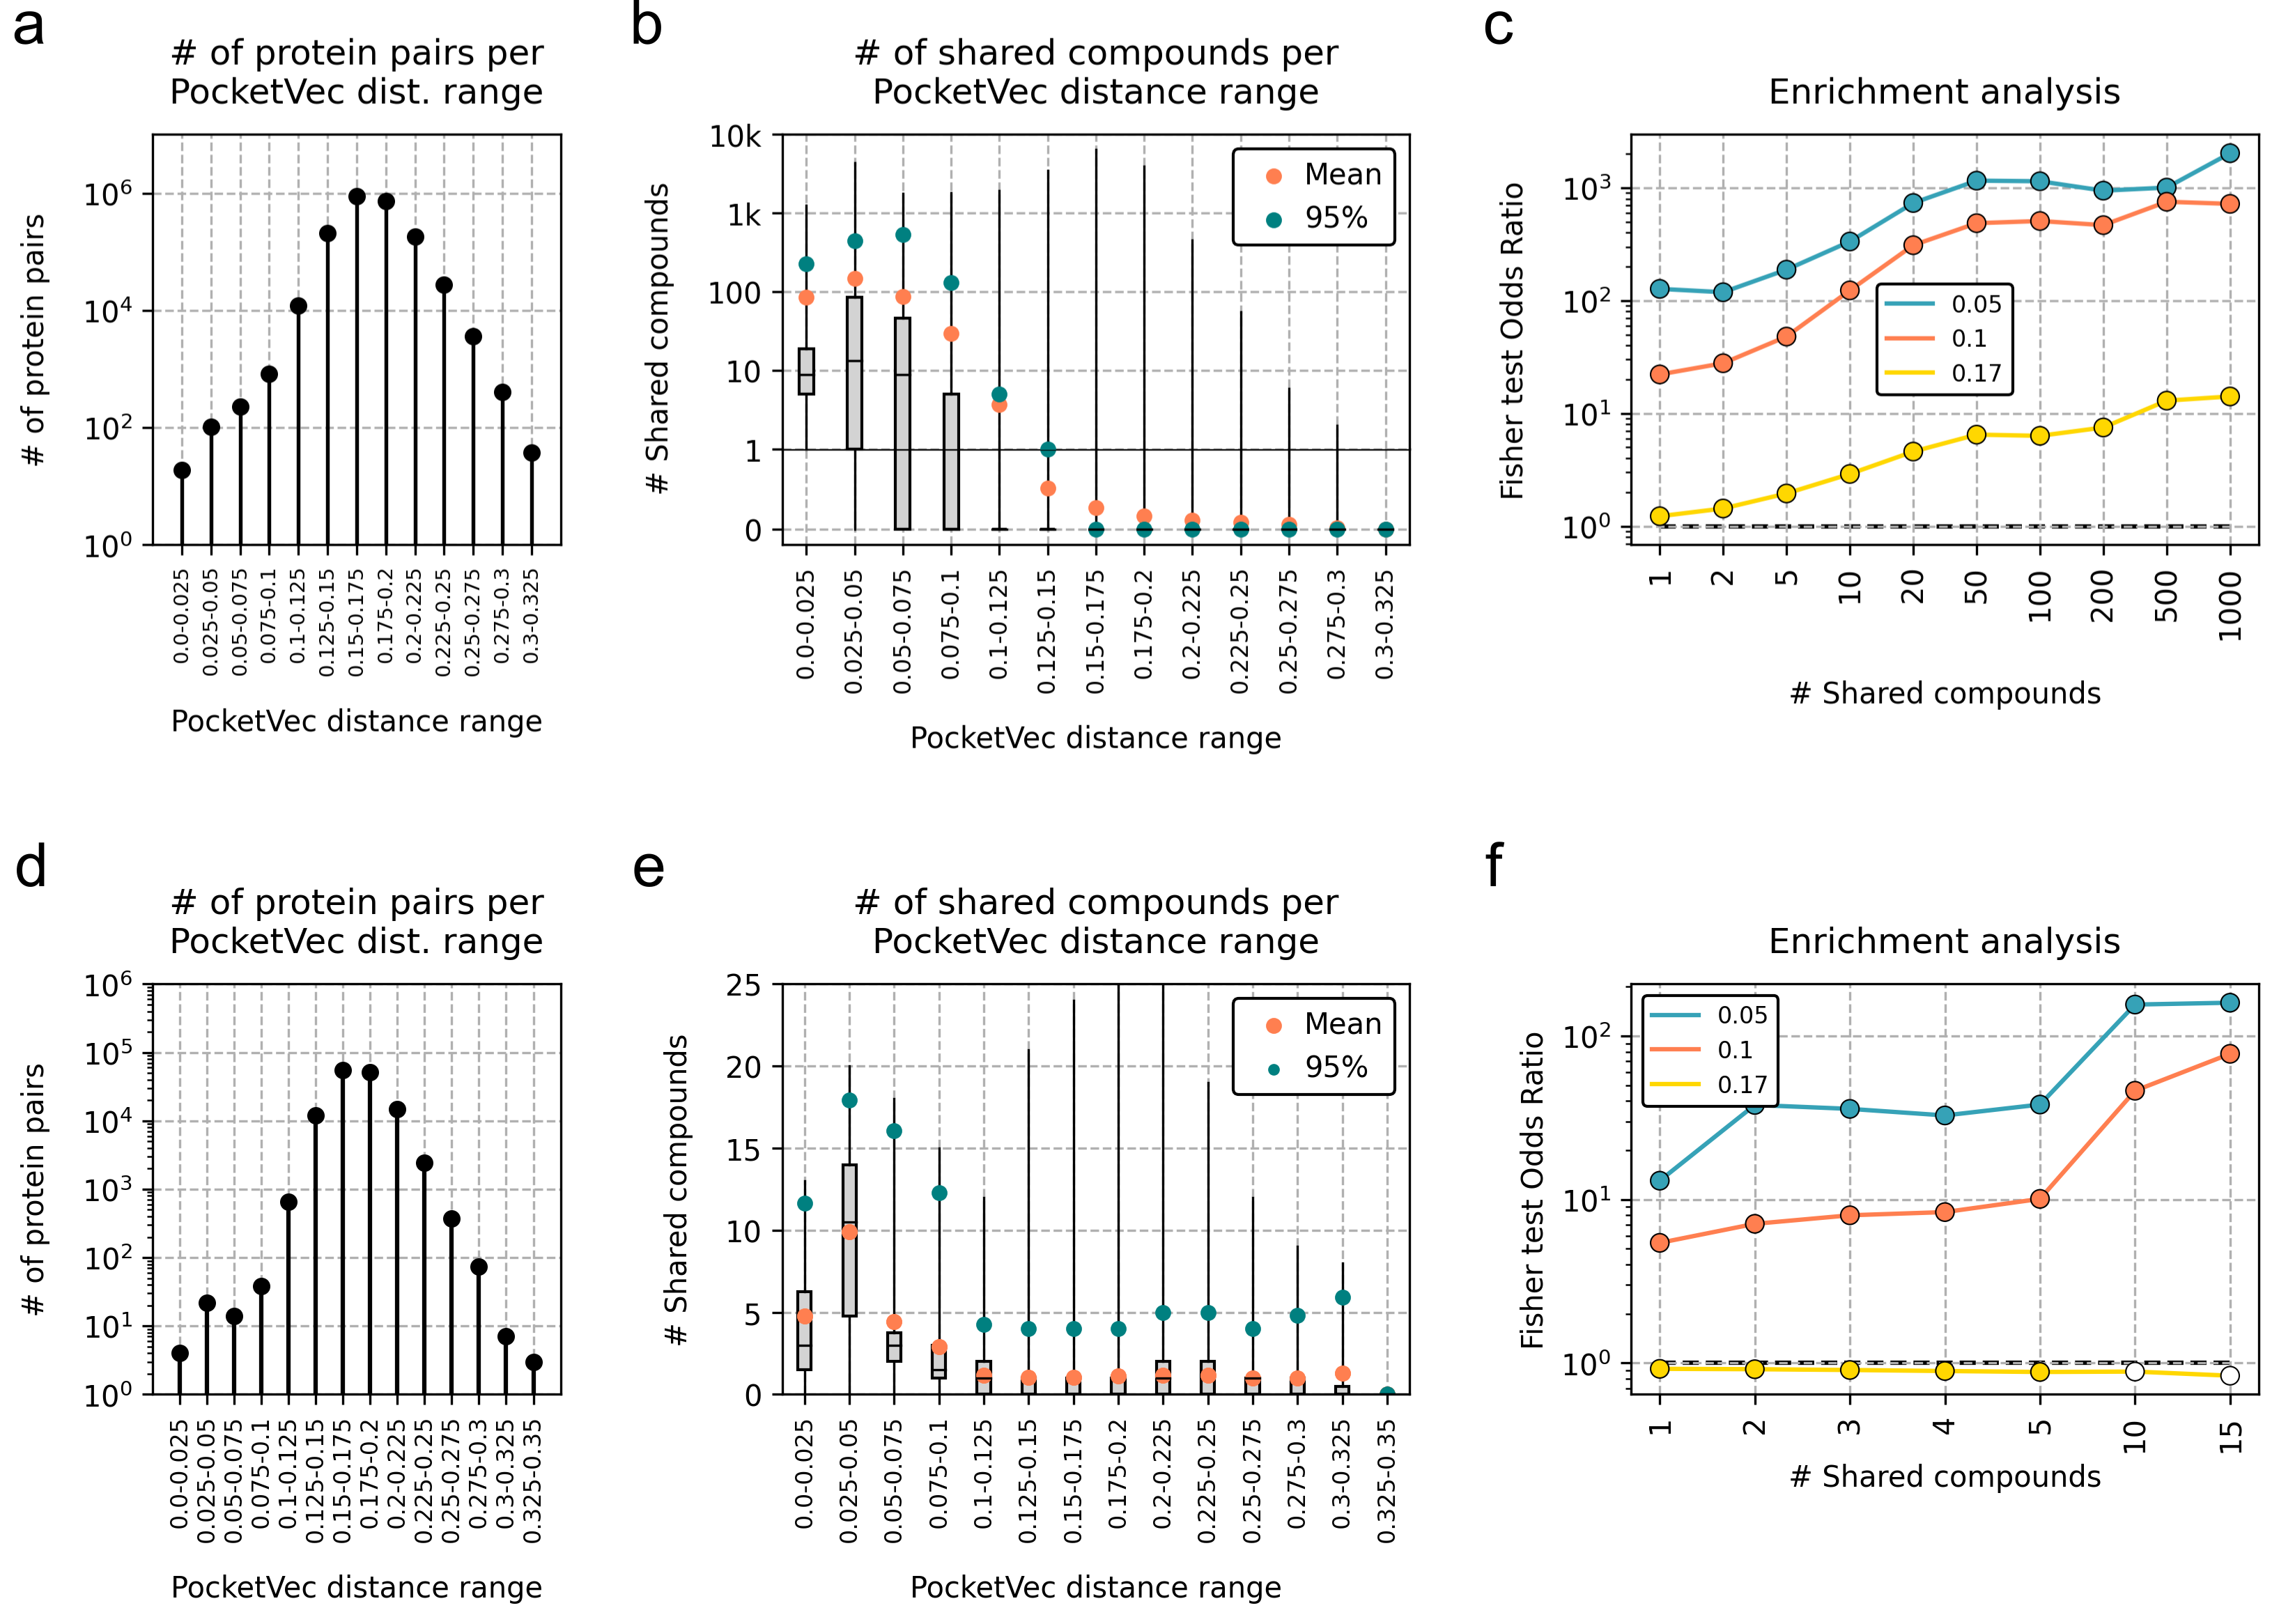
\includegraphics[width=\linewidth]{figures/PocketVec/Main/Fig6.png} 
  \caption{
    \textbf{Relationship between PocketVec similarity and experimentally determined compound-target pairs.}
    All vs All (PDB-LIG, PDB-PD, AF2-LIG and AF2-PD) comparison between PocketVec distance and number of shared compounds among proteins having experimental binding data in ChEMBL and BindingDB (a, b, c) and Offensperger et al.\cite{offensperger_large-scale_2024} (d, e, f).
    \textbf{a, d)} Number of protein pairs (y-axis) at each PocketVec distance range (x-axis).
    \textbf{b, e)} Number of shared compounds for all pairs having a PocketVec distance in the specified distance range. Orange dots indicate the average value while green dots indicate the lower bound for the top 5\% of the pairs. Boxplots indicate median (middle line), 25th, 75th percentile (box), and maximum and minimum values (whiskers). 
    \textbf{c, f)} Evolution of Fisher test Odds Ratio (y-axis) for an increasing number of shared compounds (x-axis) using an increasing value of PocketVec distance cut-off (0.05, 0.10 and 0.17). Colored dots indicate pvalue <0.001, gray dots indicate pvalue <0.05 and white dots indicate pvalue >0.05.
  }
  \label{PocketVec_Fig6}
\end{figure}

%%%%%%%%%%%%%%%%%%%%%%%%%%%%%%%%%%%%%%%%%%%%%%%%%%%%%%%%%%%%%%%%
%%% Identifying kinases with similar inhibition profiles through PocketVec descriptors
%%%%%%%%%%%%%%%%%%%%%%%%%%%%%%%%%%%%%%%%%%%%%%%%%%%%%%%%%%%%%%%%

\phantomsection
\subsubsection{Identifying kinases with similar inhibition profiles through PocketVec descriptors}
\label{PocketVec_ResultsAndDiscussion_Identifying_Kinases}

Protein kinases have long been a cornerstone of drug discovery efforts primarily due to their role as oncogenic targets\cite{attwood_trends_2021}. Since the breakthrough FDA-approval of imatinib in 2001, dozens of small molecules (72 as of November 2022\cite{roskoski_properties_2023}) have been approved as therapeutic kinase inhibitors for clinical use. However, the design of selective inhibitors is a challenging task due to the highly conserved ATP-binding pocket shared among human kinases. Indeed, many kinase inhibitors show high promiscuity (i.e. they bind to many kinases), while others are rather selective\cite{karaman_quantitative_2008, davis_comprehensive_2011}. This same variability is also apparent from the kinase perspective: some bind to many inhibitors while others are extremely selective\cite{hanson_what_2019}. Our characterization of druggable pockets in human proteins showed 1,286 potential binding sites within protein kinase domains. More specifically, we derived PocketVec descriptors for 229, 404, 195 and 458 pockets in the PDB-LIG, PDB-PD, AF2-LIG and AF2-PD sets, respectively. Thus, we set up to explore a potential correlation between the pockets in the different kinases and their experimentally determined small molecule inhibition profiles.

We first collected kinase-inhibitor pairs identified through systematic chemical proteomics approaches by Kuester and collaborators, where they tested interactions between 520 kinases and 243 inhibitors (2017 set)\cite{klaeger_target_2017}, and between 318 kinases and 1,183 inhibitors (2023 set)\cite{reinecke_chemical_2023}. We used a standard activity cutoff of 30nM to define binary kinase-inhibitor matrices, as recommended in Pharos 17 (\hyperlink{http://pharos.nih.gov}{http://pharos.nih.gov}). In the 2017 set, we found interactions involving 111 kinases and 94 inhibitors (Fig \ref{PocketVec_Fig7}a), with 43 kinases being inhibited by a single compound, and 18 of them interacting with 5 or more inhibitors (Fig \ref{PocketVec_FigS29}a). In the 2023 set, we identified interactions comprising 73 kinases and 164 inhibitors, where 19 kinases interacted with 1 inhibitor and 27 with 5 or more (Fig \ref{PocketVec_FigS29}b). We then compared kinases on the basis of their binarized inhibition profiles (Jaccard similarity, Fig \ref{PocketVec_Fig7}d, j, upper triangular matrices), and we observed that a relatively small fraction of kinase pairs shared at least 1 inhibitor (12.3\% and 9.7\% for the 2017 and 2023 sets, respectively). We also compared the kinases using PocketVec descriptors (Fig \ref{PocketVec_Fig7}d, j, lower triangular matrices), finding that the fraction of kinase pairs showing similar druggable pockets (i.e. PocketVec distances <0.17) was 40.5\% and 41.4\%, respectively. As expected, these fractions were significantly higher than the figure obtained when comparing random sets of pocket descriptors (\textasciitilde2\%. Fisher’s exact test, OR >30, p-value \textasciitilde0), since all kinases contain at least one similar ATP-binding pocket. Reassuringly, as observed in the general analysis of human druggable pockets (Fig \ref{PocketVec_Fig3}h), we found that the higher the number of common inhibitors between pairs of kinases, the more similar their pockets were according to PocketVec descriptors (Fig \ref{PocketVec_Fig7}b, h). However, even when no shared inhibitor was found for a pair of kinases, as expected, the similarity between their ATP-binding pockets was quite remarkable, suggesting that the PocketVec distance threshold should be lowered to disentangle drug promiscuity.


%%%%%%%%%%%%%%%%
%%% FIGURE 7 %%%
%%%%%%%%%%%%%%%%

% \begin{figurehere}
%   \centering
%   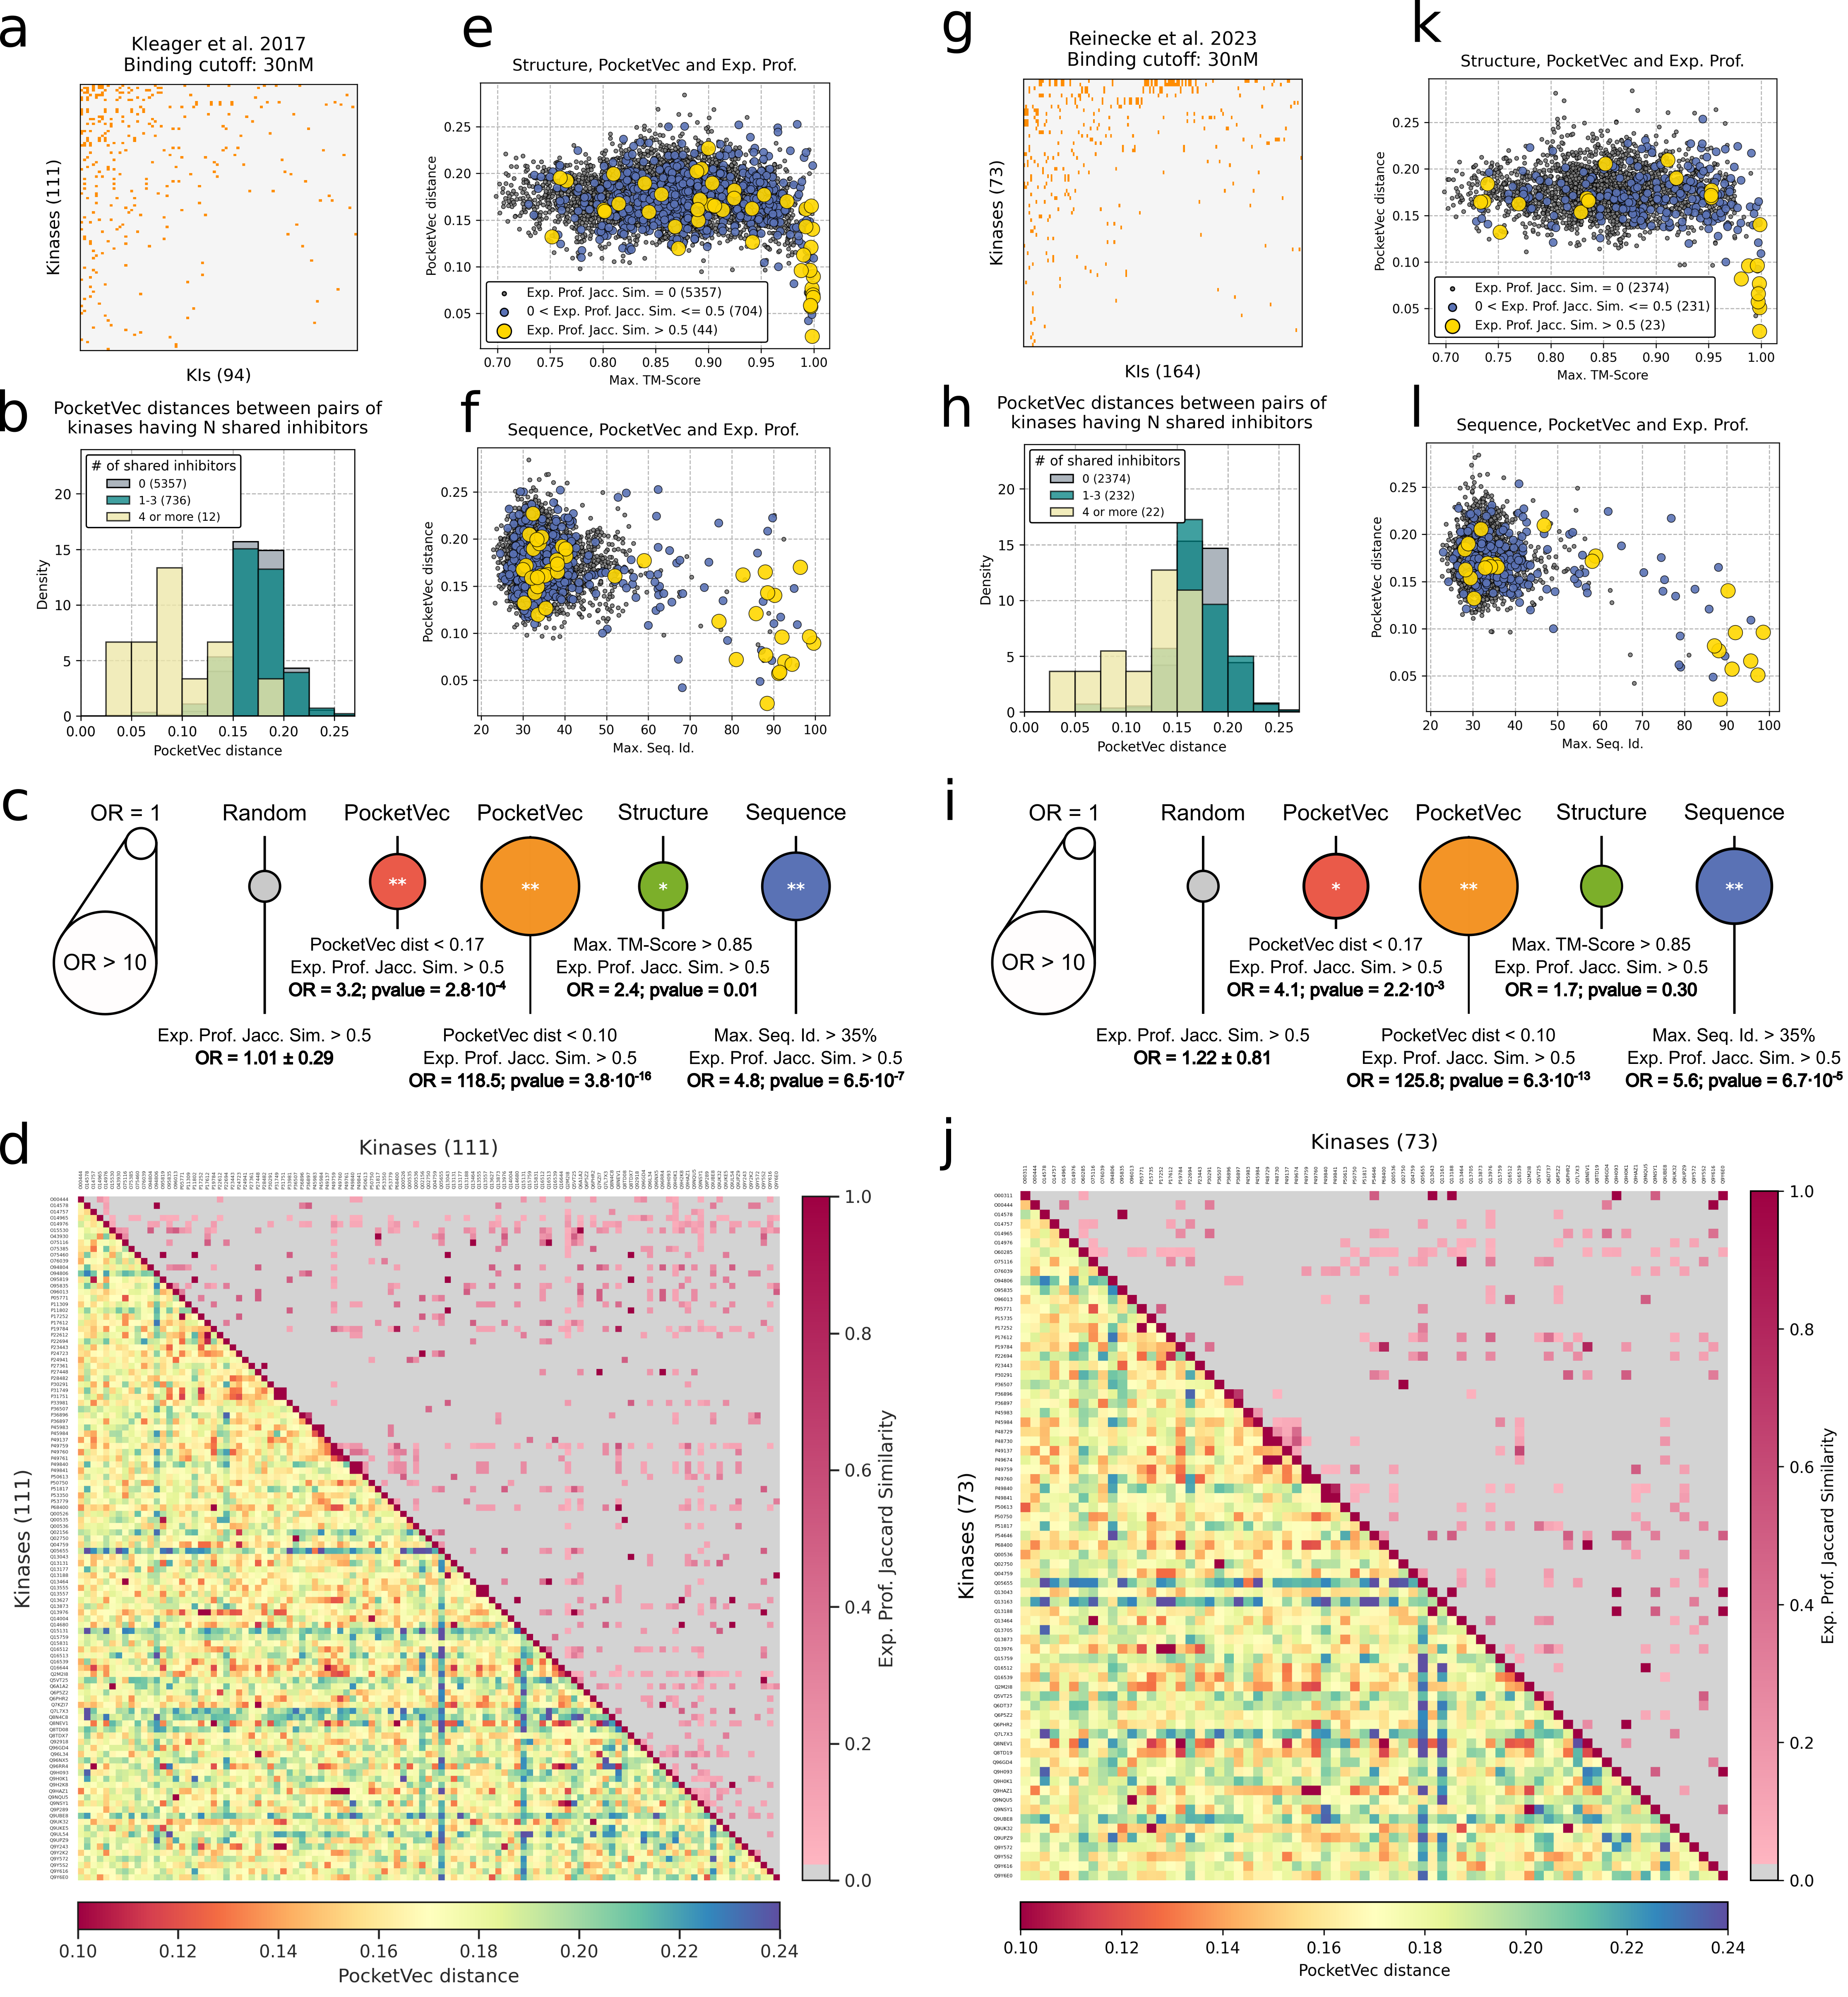
\includegraphics[width=0.8\linewidth]{figures/PocketVec/Main/Fig7.png} 
%   \caption{
%     Correlation between inhibition profiles and PocketVec descriptors. All the analyses have been performed on the data obtained from Kleager et al.\cite{klaeger_target_2017} (right panels) and Reinecke et al.\cite{reinecke_chemical_2023} (left panels).
%     \textbf{a, g)} Inhibition matrix between protein kinases, and small molecule kinase inhibitors binarized at 30 nM. Both kinases and inhibitors are sorted by the number of active inhibition events. Orange dots indicate inhibition and white dots indicate no inhibition.
%     \textbf{b, h)} Distributions of PocketVec distances grouped by the number of shared inhibitors between kinases (0, 1-3 and 4 or more). The number of kinase pairs per number of shared inhibitors is specified in parenthesis.
%     \textbf{c, i)} Enrichments (Fisher’s exact test) in similar inhibition profiles (Jaccard Similarity >0.5) for those kinase pairs being similar in terms of PocketVec distance (red: <0.17, orange: <0.10), structural similarity (TM-score >0.85) and sequence identity (>35\%). For comparison, the results obtained with randomly selected kinase pairs (gray) are also included. Circle areas are proportional to the corresponding ORs and p-values are specified in the center with the following format: * p-value < 0.05, ** p-value < 0.001.
%     \textbf{d, j)} Pairwise kinase comparisons. Rows and columns correspond to alphabetically sorted kinases (by Uniprot ID). Upper triangular matrices: kinases are compared on the basis of their experimentally determined inhibition profiles. Each square represents the Jaccard similarity between the inhibition profiles of two targets: the higher the Jaccard similarity, the more similar the corresponding inhibition profiles. Lower triangular matrices: kinases are compared on the basis of their PocketVec descriptors (employing the minimum distance among all PocketVec descriptors in the Protein Kinase Domains). The color of each square indicates the minimum PocketVec distance between two targets: the lower the PocketVec distance (red), the more similar the kinases are at pocket level according to our descriptors.
%     \textbf{e, k)} Relationship between structural similarity (x-axis, Max. TM-score) and PocketVec distances (y-axis) between pairs of protein kinases. Each point represents a kinase pair and is colored and sized in terms of the similarity between experimentally determined inhibition profiles.
%     \textbf{f, l)} Relationship between sequence similarity (x-axis, Max. Seq. Id.) and PocketVec distances (y-axis) between pairs of protein kinases. Each point represents a kinase pair and is colored and sized in terms of the similarity between experimentally determined inhibition profiles.
%     \label{PocketVec_Fig7}
%   }
% \end{figurehere}

\begin{figurehere}
 \begin{center}
  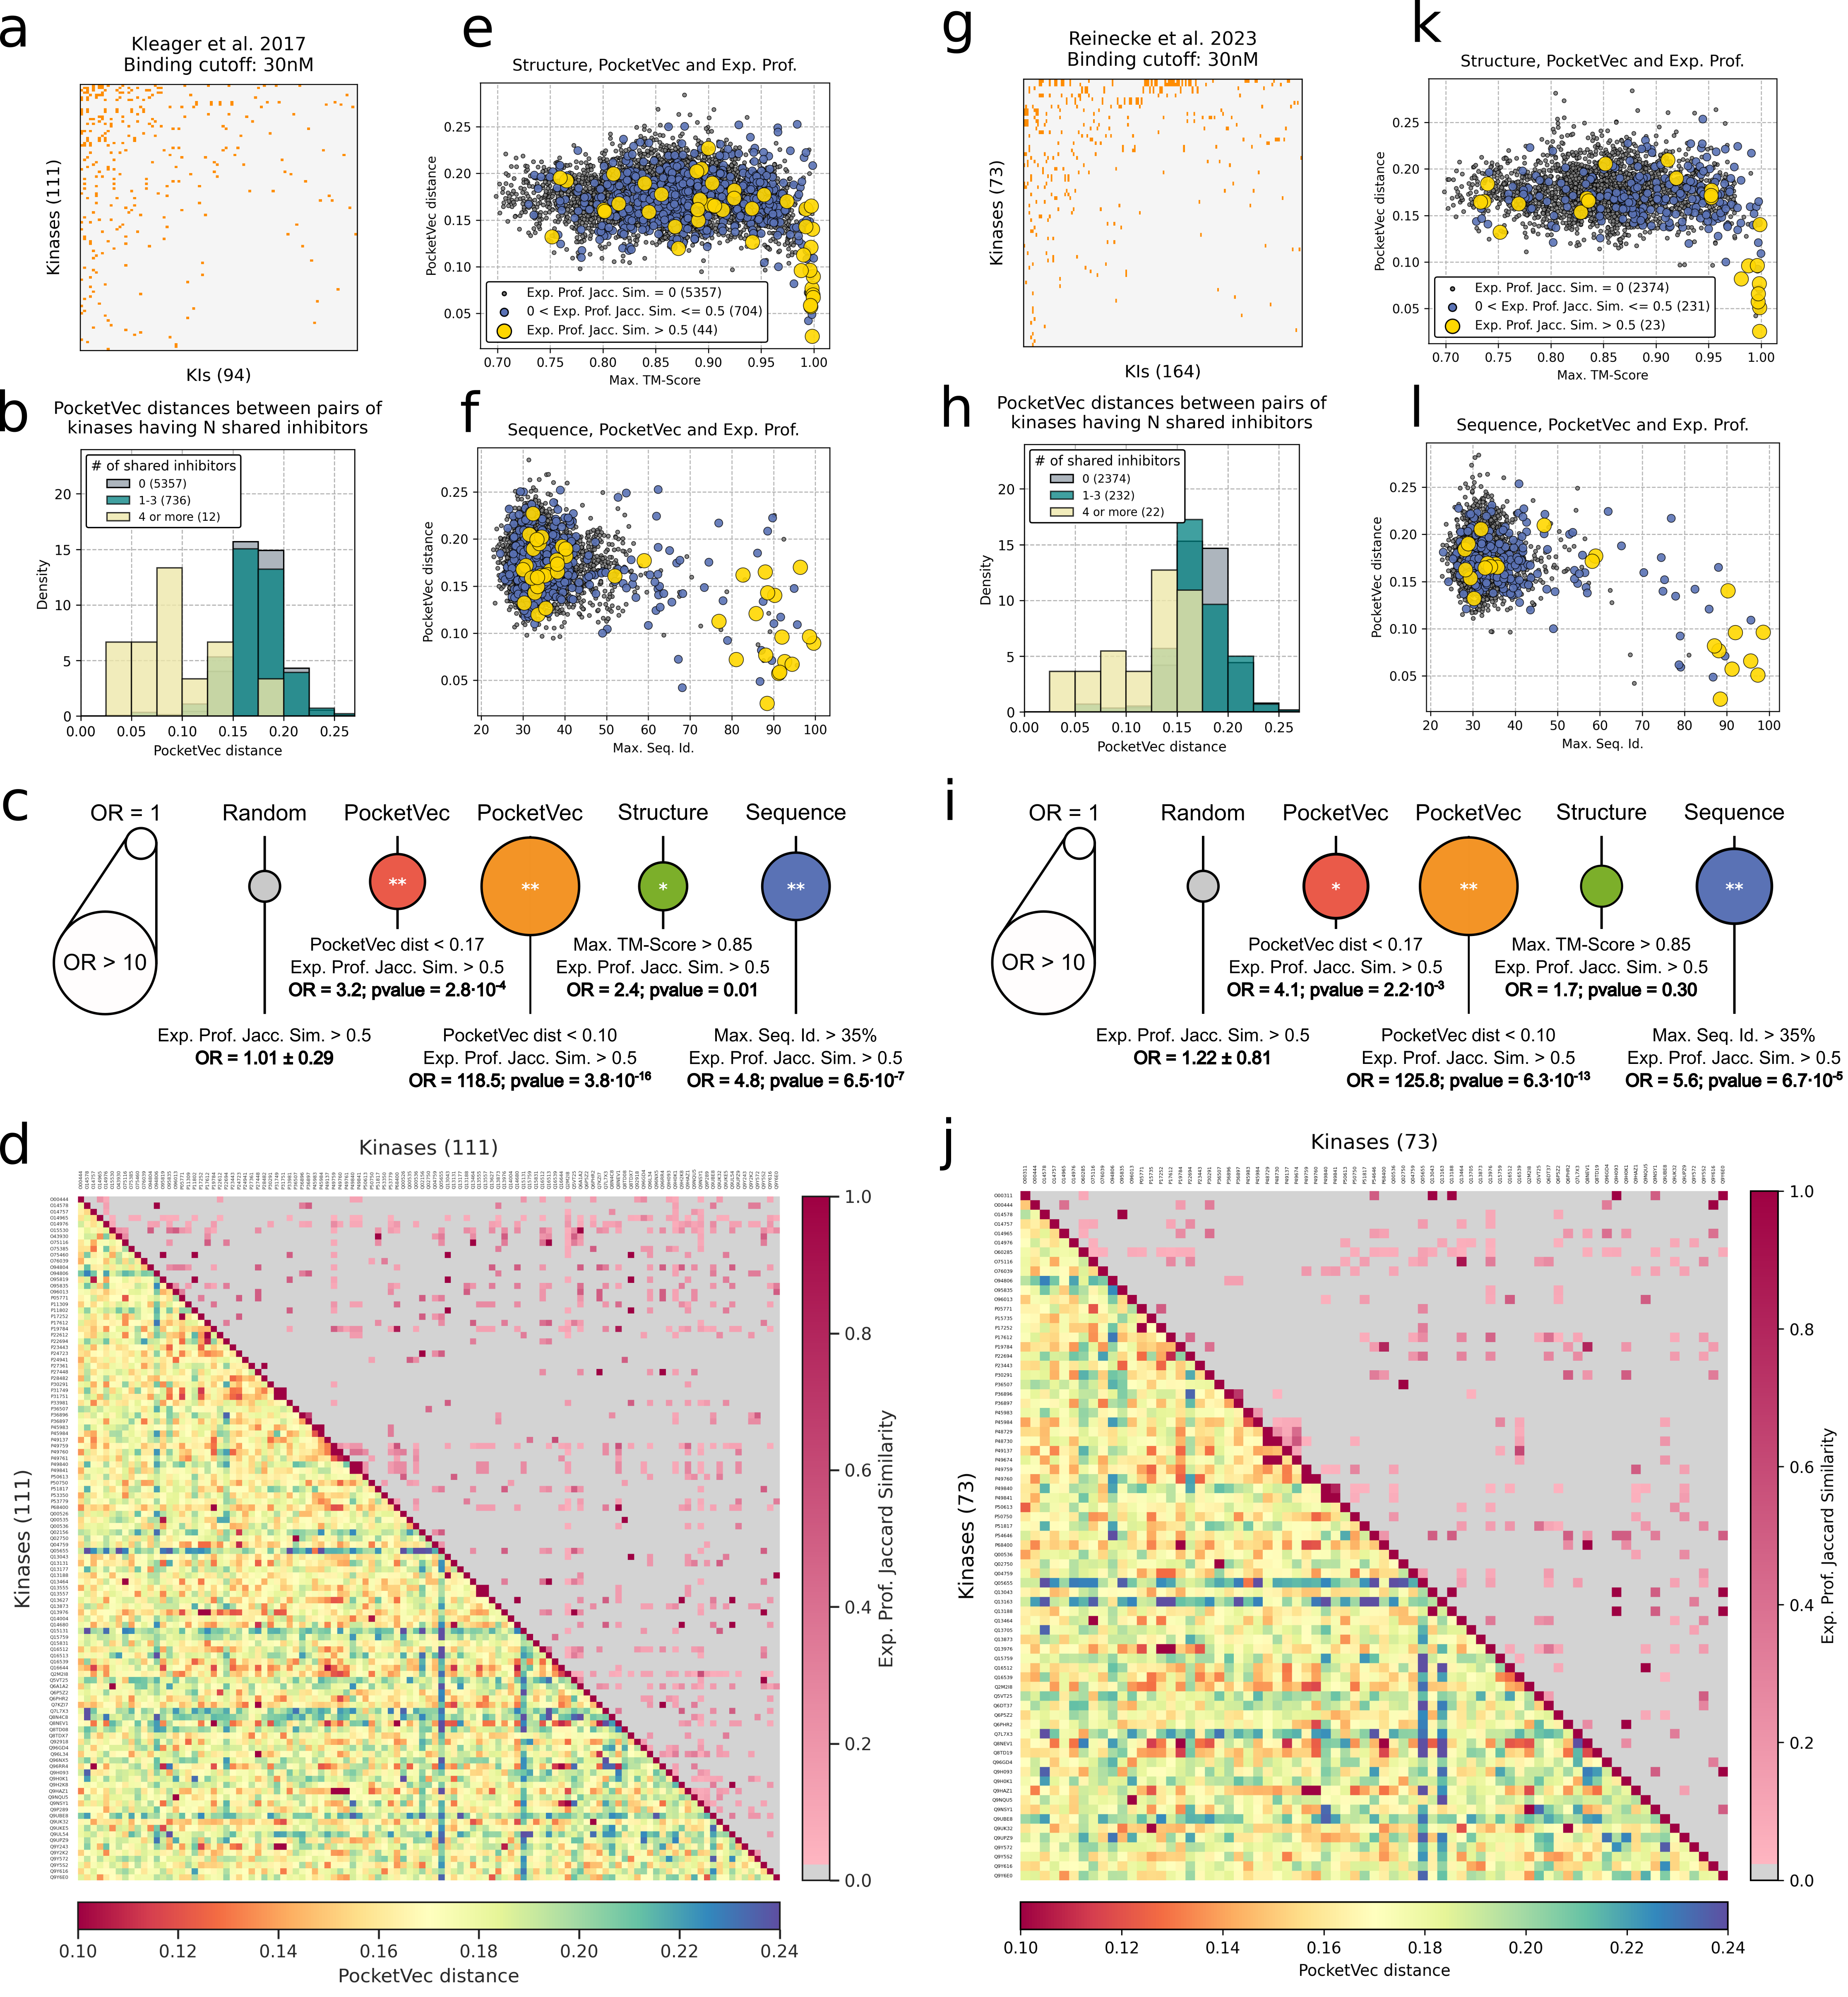
\includegraphics[width=0.7\textwidth]{figures/PocketVec/Main/Fig7.png}
  \caption{Correlation between inhibition profiles and PocketVec descriptors. All the analyses have been performed on the data obtained from Kleager et al.\cite{klaeger_target_2017} (right panels) and Reinecke et al.\cite{reinecke_chemical_2023} (left panels).
    \textbf{a, g)} Inhibition matrix between protein kinases, and small molecule kinase inhibitors binarized at 30 nM. Both kinases and inhibitors are sorted by the number of active inhibition events. Orange dots indicate inhibition and white dots indicate no inhibition.
    \textbf{b, h)} Distributions of PocketVec distances grouped by the number of shared inhibitors between kinases (0, 1-3 and 4 or more). The number of kinase pairs per number of shared inhibitors is specified in parenthesis.
    \textbf{c, i)} Enrichments (Fisher’s exact test) in similar inhibition profiles (Jaccard Similarity >0.5) for those kinase pairs being similar in terms of PocketVec distance (red: <0.17, orange: <0.10), structural similarity (TM-score >0.85) and sequence identity (>35\%). For comparison, the results obtained with randomly selected kinase pairs (gray) are also included. Circle areas are proportional to the corresponding ORs and p-values are specified in the center with the following format: * p-value < 0.05, ** p-value < 0.001.
    \textbf{d, j)} Pairwise kinase comparisons. Rows and columns correspond to alphabetically sorted kinases (by Uniprot ID). Upper triangular matrices: kinases are compared on the basis of their experimentally determined inhibition profiles. Each square represents the Jaccard similarity between the inhibition profiles of two targets: the higher the Jaccard similarity, the more similar the corresponding inhibition profiles. Lower triangular matrices: kinases are compared on the basis of their PocketVec descriptors (employing the minimum distance among all PocketVec descriptors in the Protein Kinase Domains). The color of each square indicates the minimum PocketVec distance between two targets: the lower the PocketVec distance (red), the more similar the kinases are at pocket level according to our descriptors.
    \textbf{e, k)} Relationship between structural similarity (x-axis, Max. TM-score) and PocketVec distances (y-axis) between pairs of protein kinases. Each point represents a kinase pair and is colored and sized in terms of the similarity between experimentally determined inhibition profiles.
    \textbf{f, l)} Relationship between sequence similarity (x-axis, Max. Seq. Id.) and PocketVec distances (y-axis) between pairs of protein kinases. Each point represents a kinase pair and is colored and sized in terms of the similarity between experimentally determined inhibition profiles.
 }
 \label{PocketVec_Fig7}
 \end{center}
\end{figurehere}
  

Next, we parsed the general inhibition matrices to derive inhibition profiles for each kinase (i.e. a vector describing whether it does or does not interact with every tested inhibitor), and we assessed the coherence between PocketVec distances and the similarity between experimentally determined inhibition profiles. Indeed, kinase pairs with low PocketVec distances (<0.17) showed a significant enrichment for similar inhibition profiles (Fisher’s exact test, OR = 3.2, p-value <0.0003 in the 2017 set, and OR = 4.1, p-value <0.003 in the 2023 set for a Jaccard similarity >0.5). These enrichments were even more pronounced when we applied more stringent distance thresholds (PocketVec distance <0.10) with OR >118 and OR >125 (p-values <10\textsuperscript{-10}) for the 2017 and 2023 sets, respectively (Fig \ref{PocketVec_Fig7}c, i).

We then compared our results using PocketVec descriptors to more classical structure and sequence similarity analyses (see \hyperref[PocketVec_Methods]{Methods}). As expected, we found that structurally similar proteins (Max. TM-score >0.85) were also moderately enriched in similar inhibition profiles (OR = 2.4, p-value <0.05; OR = 1.7, p-value >0.05), as were kinases sharing >35\% sequence identity (OR = 4.8, p-value <10\textsuperscript{-6}; OR = 5.5, p-value <10\textsuperscript{-4}). Finally, we studied the relationship between structure, sequence, PocketVec and inhibition profile similarity between kinase pairs. Consistently with our global analysis of the human druggable pockets (Fig \ref{PocketVec_Fig5}a), higher structure and sequence similarities consistently led to lower PocketVec distances in both the 2017 (Fig \ref{PocketVec_Fig7}e, f) and the 2023 (Fig \ref{PocketVec_Fig7}k, l) sets.

Despite the coherence of the results of the three metrics, interestingly, we found 9 kinase pairs (4 in the 2017 and 5 in the 2023 sets) with clear inhibition profile similarities that only PocketVec descriptors could pick. On the other hand, our analyses also revealed 8 cases (5 in the 2017 and 3 in the 2023 sets) where PocketVec descriptors fell short to detect similarities that could be recovered by sequence or structure comparisons alone. Overall, these results emphasize the coherence and complementarity between strategies, highlighting the potential of PocketVec descriptors to identify otherwise unattainable similarities in experimental inhibition profiles among protein kinases. 